
\documentclass[11pt,a4paper]{article}
\usepackage[T1]{fontenc}
\usepackage[utf8]{inputenc}
\usepackage{newtxtext,newtxmath}
\usepackage{amsmath,mathtools}
\usepackage[a4paper,margin=1in]{geometry}
\usepackage{setspace}
\usepackage{titlesec}
\usepackage{enumitem}
\usepackage{booktabs,array,longtable,tabularx,multirow}
\usepackage{xcolor}
\usepackage{hyperref}
\usepackage{tcolorbox}
\usepackage{listings}
\usepackage{fancyhdr}
\usepackage{lastpage}
\usepackage{microtype}
\usepackage{tikz}
\usetikzlibrary{arrows.meta,positioning,shapes.geometric}
\tcbuselibrary{breakable,skins}
\definecolor{DeepBlue}{RGB}{20,42,92}
\definecolor{SoftBlue}{RGB}{239,246,255}
\definecolor{SoftGray}{RGB}{247,247,247}
\definecolor{CodeGray}{RGB}{248,248,248}
\definecolor{DarkGreen}{RGB}{0,100,80}
\hypersetup{colorlinks=true,linkcolor=DeepBlue,citecolor=DeepBlue,urlcolor=DeepBlue}
\setstretch{1.13}
\setlength{\parskip}{0.45em}
\setlength{\parindent}{0pt}
\setlist[itemize]{leftmargin=1.4em,itemsep=0.2em,topsep=0.2em}
\setlist[enumerate]{leftmargin=1.6em,itemsep=0.2em,topsep=0.2em}
\titleformat{\section}{\normalfont\Large\bfseries}{\thesection.}{0.6em}{}
\titleformat{\subsection}{\normalfont\large\bfseries}{\thesubsection}{0.6em}{}
\titleformat{\subsubsection}{\normalfont\normalsize\bfseries}{\thesubsubsection}{0.6em}{}
\pagestyle{fancy}
\fancyhf{}
\lhead{\small\leftmark}
\rhead{\small\thepage/\pageref{LastPage}}
\renewcommand{\headrulewidth}{0.4pt}
\newcommand{\R}{\mathbb{R}}
\newcommand{\E}{\mathbb{E}}
\newcommand{\dd}{\mathrm{d}}
\newcommand{\argmin}{\operatorname*{arg\,min}}
\newcommand{\argmax}{\operatorname*{arg\,max}}
\newcommand{\softmax}{\operatorname{softmax}}
\newcommand{\sigmoid}{\operatorname{sigmoid}}
\newcommand{\softplus}{\operatorname{softplus}}
\newcommand{\clip}{\operatorname{clip}}
\newcommand{\norm}[1]{\left\lVert #1 \right\rVert}
\newcommand{\policy}{\pi}
\newcommand{\Hamilton}{\mathcal{H}}
\newcommand{\Loss}{\mathcal{L}}
\newtcolorbox{definitionbox}{breakable,enhanced,colback=SoftBlue,colframe=DeepBlue,boxrule=0.6pt,arc=2pt,left=6pt,right=6pt,top=5pt,bottom=5pt}
\newtcolorbox{remarkbox}{breakable,enhanced,colback=SoftGray,colframe=black!55,boxrule=0.5pt,arc=2pt,left=6pt,right=6pt,top=5pt,bottom=5pt}
\newtcolorbox{workflowbox}{breakable,enhanced,colback=white,colframe=DarkGreen,boxrule=0.6pt,arc=2pt,left=6pt,right=6pt,top=5pt,bottom=5pt}
\lstdefinestyle{pythonstyle}{language=Python,basicstyle=\ttfamily\footnotesize,backgroundcolor=\color{CodeGray},breaklines=true,columns=fullflexible,frame=single,showstringspaces=false,keywordstyle=\color{DeepBlue}\bfseries,commentstyle=\color{black!55},stringstyle=\color{DarkGreen},numbers=left,numberstyle=\tiny\color{black!45},xleftmargin=1em,framexleftmargin=1em}
\newcommand{\lecturetitle}[4]{%
\begin{titlepage}
\centering
\vspace*{2.3cm}
{\bfseries\LARGE #1\par}
\vspace{0.6cm}
{\Large #2\par}
\vspace{1.4cm}
{\large #3\par}
\vfill
{\large #4\par}
\vspace{1.0cm}
\end{titlepage}}
% Compatibility aliases for earlier note versions
\newcommand{\ODESolve}{\operatorname{ODESolve}}
\newcommand{\ind}{\mathbf{1}}
\newenvironment{boxednote}{\begin{definitionbox}}{\end{definitionbox}}
\newenvironment{methodbox}{\begin{remarkbox}}{\end{remarkbox}}
\newenvironment{flowbox}{\begin{workflowbox}\centering}{\end{workflowbox}}
\newenvironment{keybox}[1]{\begin{definitionbox}\textbf{#1.}\ }{\end{definitionbox}}
\newenvironment{takeaway}{\begin{keybox}{Takeaway}}{\end{keybox}}
\newenvironment{warningbox}{\begin{keybox}{Caution}}{\end{keybox}}
\newenvironment{examplebox}[1]{\begin{keybox}{Example: #1}}{\end{keybox}}

\begin{document}
\lecturetitle{Lecture Note 2}{PINN and PIDL for Cyber Propagation, Parameter Learning, and Optimal Control}{A self-contained tutorial with implementation details, evaluation guidance, and Python examples}{Prepared for advanced research discussion and supervision}
\tableofcontents
\newpage
\section*{Reading Guide}
\addcontentsline{toc}{section}{Reading Guide}
This lecture note is designed to be self-contained. It does not assume that the reader has read a separate note on reinforcement learning, differential games, or Pontryagin's Maximum Principle. The main focus is \emph{Physics-Informed Neural Networks} (PINNs) and the broader family of \emph{Physics-Informed Deep Learning} (PIDL) methods for cyber propagation systems. PINN is treated as the core method; PIDL is introduced as the larger design philosophy that combines neural networks, differential-equation knowledge, partial observations, priors, simulators, and sometimes optimality or game-theoretic conditions.

The note answers four practical questions.
\begin{enumerate}[leftmargin=2em]
    \item What is a PINN and what problem does it solve?
    \item How can a PINN learn unknown propagation parameters from sparse or noisy data?
    \item How can a PINN be used to solve optimal control problems for malware, APT, rumor, or misinformation dynamics?
    \item How does PIDL extend PINN when the model is only partially known, when extra priors are available, or when we need to combine differentiable simulation with neural learning?
    \item What are the implementation choices that make a PINN work in practice: network outputs, collocation points, automatic differentiation, constrained parameters, loss balancing, and validation?
\end{enumerate}

The note deliberately separates \emph{modeling}, \emph{learning}, \emph{control}, and \emph{validation}. This is important because many papers mix these concepts. A clear PINN study should state: the differential equation model, the available data, the unknown quantities, the neural networks used to approximate them, the residuals included in the loss, and the criteria used to validate the result.

\begin{takeaway}
A PINN is not merely a neural network fitted to data. It is a neural approximation whose training loss includes residuals of differential equations, boundary/initial conditions, conservation laws, and sometimes optimality conditions. In cyber propagation research, this allows us to combine limited data with prior mechanistic knowledge about spreading dynamics.

\end{takeaway}

\section*{Core Notation}
\addcontentsline{toc}{section}{Core Notation}
\begin{longtable}{p{0.18\linewidth}p{0.74\linewidth}}
\toprule
Symbol & Meaning \\
\midrule
$t\in[0,T]$ & Continuous time over the modeling or control horizon. \\
$x(t)$ & State vector, such as malware compartments, APT states, or opinion states. \\
$u(t)$ & Control function, such as patching, monitoring, education, or counter-messaging intensity. \\
$\theta$ & Unknown or partially known physical/cyber parameters, such as infection and recovery rates. \\
$f(x,u,\theta,t)$ & Right-hand side of the differential equation. It encodes the assumed propagation mechanism. \\
$N_x(t;\phi)$ & Neural network with parameters $\phi$ used to approximate the state trajectory $x(t)$. \\
$N_u(t;\psi)$ & Neural network used to approximate a control function $u(t)$, when control is learned. \\
$N_\lambda(t;\eta)$ & Neural network used to approximate the costate $\lambda(t)$ in PMP-informed PINNs. \\
$t_i^d$ & Data points where observations are available. \\
$t_j^f$ & Collocation points where equation residuals are enforced. \\
$r_f(t)$ & Differential equation residual. Small residual means the neural trajectory approximately satisfies the model. \\
$\mathcal{L}$ & Training loss, usually a weighted sum of data, residual, boundary, constraint, and control terms. \\
\bottomrule
\end{longtable}

\section{Why PINNs for Cyber Propagation?}

Cybersecurity propagation models often have a mechanistic structure. Examples include malware spreading in Internet-of-Things networks, APT compromise and recovery, rumor diffusion, misinformation propagation, and propaganda/counter-propaganda dynamics. These topics are closely related to recent cyber control studies on malware optimal control, APT security evaluation, and hybrid propaganda-war games \cite{jafar2024malware,yang2019apt,cheng2024hodge}. A generic compartment model has the form
\begin{equation}
    \dot{x}(t)=f(x(t),u(t),\theta,t), \qquad x(0)=x_0,
    \label{eq:generic_ode}
\end{equation}
where:
\begin{itemize}[leftmargin=2em]
    \item $x(t)\in\R^n$ is the state, such as susceptible, infected, and recovered proportions, or unaware, propaganda, and counter-propaganda proportions;
    \item $u(t)\in\R^m$ is a control input, such as patching, monitoring, education, isolation, or counter-messaging intensity;
    \item $\theta$ is a vector of propagation parameters, such as infection rates, recovery rates, forgetting rates, and intervention efficacy coefficients;
    \item $f$ encodes the assumed propagation mechanism.
\end{itemize}

A conventional workflow is:
\begin{center}
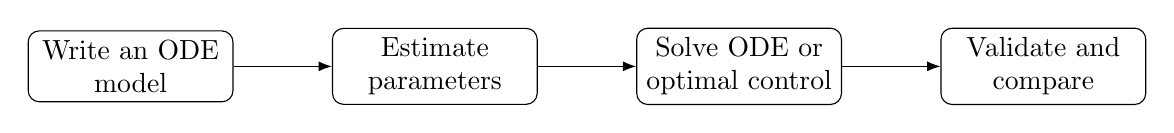
\begin{tikzpicture}[node distance=1.25cm,>=Latex]
\tikzstyle{box}=[rectangle,rounded corners,draw=black,align=center,minimum width=2.6cm,minimum height=0.9cm]
\node[box] (model) {Write an ODE\\model};
\node[box,right=of model] (param) {Estimate\\parameters};
\node[box,right=of param] (solve) {Solve ODE or\\optimal control};
\node[box,right=of solve] (eval) {Validate and\\compare};
\draw[->] (model) -- (param);
\draw[->] (param) -- (solve);
\draw[->] (solve) -- (eval);
\end{tikzpicture}
\end{center}

This workflow is effective when data are abundant and the numerical problem is easy. However, cyber propagation studies often face three difficulties.
\begin{enumerate}[leftmargin=2em]
    \item \textbf{Sparse data.} We may only observe infected nodes, not all compartments. Data can be noisy, delayed, aggregated, or simulated.
    \item \textbf{Unknown or partially known parameters.} Attack and defense rates are not directly observable.
    \item \textbf{Control and game objectives.} We often want not only to fit historical data, but also to compute an optimal defense policy under cost constraints.
\end{enumerate}

PINNs address these difficulties by training neural networks under both data and physics constraints. The original PINN framework was popularized by Raissi, Perdikaris, and Karniadakis \cite{raissi2019pinn}; broad reviews and extensions are provided in \cite{karniadakis2021pinnreview,lu2021deepxde}. For high-dimensional PDEs, related neural PDE solvers such as the Deep Galerkin Method were proposed by Sirignano and Spiliopoulos \cite{sirignano2018dgm}. For continuous-time learned dynamics, Neural ODEs \cite{chen2018neuralode} are closely related, but their purpose is different: Neural ODEs typically learn the right-hand side of the differential equation, while PINNs enforce a known or partially known differential equation through residuals.

\subsection{What a PINN contributes in this setting}
A PINN can support at least four tasks:
\begin{enumerate}[leftmargin=2em]
    \item \textbf{Forward solution:} approximate $x(t)$ when $\theta$ and $u(t)$ are known.
    \item \textbf{Inverse parameter learning:} estimate unknown $\theta$ from sparse observations.
    \item \textbf{Direct neural control:} learn an open-loop control function $u(t)$ by minimizing a cost subject to the dynamics.
    \item \textbf{PMP-informed control:} learn state, costate, and control functions by embedding the optimality system derived from Pontryagin's Maximum Principle (PMP) into the loss.
\end{enumerate}

These tasks are related but not identical. A common source of confusion is to call all of them ``PINN control''. This note separates them carefully.

\subsection{A clearer taxonomy of PINN tasks}
The same mathematical model can lead to different PINN formulations depending on what is known and what is unknown. The following table should be read before designing a network. It prevents a common mistake: using a single loss expression without first deciding what the unknown object actually is.

\begin{longtable}{p{0.22\linewidth}p{0.22\linewidth}p{0.24\linewidth}p{0.24\linewidth}}
\toprule
Task & Known quantities & Unknown quantities & Main loss terms \\
\midrule
Forward PINN & Model $f$, parameters $\theta$, initial condition & State trajectory $x(t)$ & ODE residual + initial/boundary conditions \\
Inverse PINN & Model form $f$, partial observations & Parameters $\theta$ and hidden states & Data loss + ODE residual + priors/constraints \\
Control PINN & Model, cost functional, constraints & Control function $u(t)$ and state $x(t)$ & Cost + ODE residual + control bounds \\
PMP-informed PINN & PMP optimality system & State, costate, control & State residual + costate residual + stationarity + boundary \\
Game-aware PINN & Game model and objectives & Multi-player controls/costates & State residual + player-wise optimality residuals + game validation \\
Hybrid/impulse PINN & ODE between events and jump map & Piecewise states/controls and impulse strengths & ODE residuals + jump residuals + event constraints \\
\bottomrule
\end{longtable}

A practical rule is: start from the simplest task that can answer the research question. If the goal is only to estimate $\beta$ and $\gamma$, do not introduce control networks. If the goal is to compute an optimal defense plan, first verify the forward and inverse PINNs, then add control. If the goal is a game, first solve or validate the single-player control version, then add player-wise Hamiltonians.

\begin{takeaway}
PINN design should begin with the sentence: ``The unknown object is ...''. The network outputs and loss terms should follow from that sentence. This simple discipline makes the method much clearer.
\end{takeaway}

\section{Mathematical Preliminaries}

\subsection{Ordinary differential equations}
A continuous-time propagation model is usually an ODE:
\begin{equation}
    \frac{\dd x}{\dd t}=f(x(t),u(t),\theta,t), \qquad t\in[0,T].
\end{equation}
The derivative $\dot{x}(t)$ describes the instantaneous rate of change. For example, if $I(t)$ is the infected proportion, then $\dot{I}(t)>0$ means infection is growing at time $t$.

A numerical ODE solver, such as Euler or Runge-Kutta, approximates the solution by stepping forward in time. A PINN instead represents $x(t)$ by a neural network $x_\phi(t)$ and uses automatic differentiation to compute $\frac{\dd x_\phi}{\dd t}$. It then penalizes the mismatch
\begin{equation}
    r_f(t)=\frac{\dd x_\phi(t)}{\dd t}-f(x_\phi(t),u(t),\theta,t).
\end{equation}
If $r_f(t)$ is small at many collocation points, then $x_\phi(t)$ approximately satisfies the ODE.

\subsection{Neural networks as function approximators}
A feedforward neural network maps an input $t$ to an output $x_\phi(t)$:
\begin{equation}
    x_\phi(t)=W_L \sigma\big(W_{L-1}\sigma(\cdots \sigma(W_1 t+b_1)\cdots)+b_{L-1}\big)+b_L,
\end{equation}
where $\phi$ collects all weights and biases. The activation function $\sigma$ is often $\tanh$, ReLU, sigmoid, or sine. For PINNs, $\tanh$ is often used because it is smooth and stable for computing derivatives.

The key PINN idea is not that neural networks are magic solvers. The key idea is that neural networks are differentiable function approximators. Automatic differentiation gives exact derivatives of the network output with respect to the input, up to floating point precision.

\subsection{Data points and collocation points}
PINN training usually uses two types of time points.
\begin{itemize}[leftmargin=2em]
    \item \textbf{Data points} $\{t_i^{d}\}_{i=1}^{N_d}$ are times where observations are available, for example $I^{obs}(t_i^d)$.
    \item \textbf{Collocation points} $\{t_j^{f}\}_{j=1}^{N_f}$ are times where the differential equation residual is enforced. They do not require observed data.
\end{itemize}

This distinction explains why PINNs are useful under limited data. Even if observations are available at only a few time points, the ODE residual can be enforced at many collocation points.

\section{The Basic PINN Formulation}

Consider the ODE
\begin{equation}
    \dot{x}(t)=f(x(t),\theta,t), \qquad x(0)=x_0.
\end{equation}
Let $x_\phi(t)$ be a neural network approximation of $x(t)$. The residual is
\begin{equation}
    r_\phi(t)=\frac{\dd x_\phi(t)}{\dd t}-f(x_\phi(t),\theta,t).
\end{equation}
A basic PINN loss is
\begin{equation}
    \mathcal{L}(\phi)=w_d\mathcal{L}_{data}+w_f\mathcal{L}_{ode}+w_0\mathcal{L}_{ic},
\end{equation}
where
\begin{align}
    \mathcal{L}_{data} &= \frac{1}{N_d}\sum_{i=1}^{N_d}\norm{x_\phi(t_i^d)-x_i^{obs}}^2,\\
    \mathcal{L}_{ode} &= \frac{1}{N_f}\sum_{j=1}^{N_f}\norm{r_\phi(t_j^f)}^2,\\
    \mathcal{L}_{ic} &= \norm{x_\phi(0)-x_0}^2.
\end{align}
Here $w_d,w_f,w_0$ are loss weights. Their values matter: if $w_f$ is too small, the network may fit data but violate the model; if $w_f$ is too large, the network may satisfy the ODE but ignore noisy observations. Loss imbalance is a known difficulty for PINNs \cite{wang2021lossimbalance,krishnapriyan2021pinnfailures}.

\begin{center}
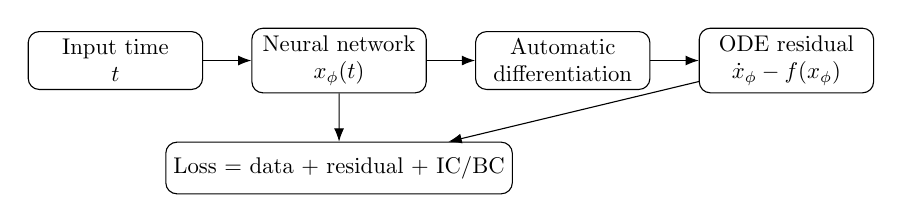
\begin{tikzpicture}[node distance=0.75cm,>=Latex,scale=0.82,transform shape]
\tikzstyle{box}=[rectangle,rounded corners,draw=black,align=center,minimum width=2.7cm,minimum height=0.8cm]
\node[box] (input) {Input time\\$t$};
\node[box,right=of input] (nn) {Neural network\\$x_\phi(t)$};
\node[box,right=of nn] (ad) {Automatic\\differentiation};
\node[box,right=of ad] (res) {ODE residual\\$\dot{x}_\phi-f(x_\phi)$};
\node[box,below=of nn] (loss) {Loss = data + residual + IC/BC};
\draw[->] (input) -- (nn);
\draw[->] (nn) -- (ad);
\draw[->] (ad) -- (res);
\draw[->] (nn) -- (loss);
\draw[->] (res) -- (loss);
\end{tikzpicture}
\end{center}

\begin{takeaway}
A PINN uses collocation points to turn a differential equation into a training signal. The network does not need data at every collocation point. It only needs the equation residual there.
\end{takeaway}

\subsection{PINN as constrained regression}
It is helpful to view a PINN as a constrained regression problem. A standard neural network tries to fit observed pairs $(t_i,x_i^{obs})$. A PINN tries to fit observed data while also remaining close to the solution manifold of a differential equation. In words,
\begin{equation}
    \text{PINN solution} = \text{data-consistent} + \text{model-consistent} + \text{constraint-consistent}.
\end{equation}
The three requirements play different roles:
\begin{itemize}[leftmargin=2em]
    \item the \emph{data loss} anchors the neural trajectory to observations;
    \item the \emph{physics residual} prevents physically implausible interpolation between sparse observations;
    \item the \emph{initial, boundary, conservation, and bound constraints} remove solutions that are mathematically allowed by the residual but impossible for the cyber system.
\end{itemize}
For example, if only $I(t)$ is observed in a malware model, the data loss alone says little about $S(t)$ and $R(t)$. The ODE residual links $S$, $I$, and $R$ through transition mechanisms, while the conservation law $S+I+R=1$ further restricts the hidden states.

\subsection{What each loss component prevents}
\begin{longtable}{p{0.22\linewidth}p{0.34\linewidth}p{0.34\linewidth}}
\toprule
Loss component & It encourages & Without it, the risk is \\
\midrule
Data loss & Agreement with observations & Smooth but wrong model-consistent curves \\
ODE residual & Agreement with the assumed dynamics & Overfitting sparse/noisy observations \\
Initial/boundary loss & Correct starting/terminal conditions & Time-shifted or boundary-inconsistent solutions \\
Conservation/positivity loss & Valid compartment proportions & Negative populations or mass imbalance \\
Parameter prior/range & Realistic learned rates & Nonphysical but numerically convenient parameters \\
Control cost & Cost-effective defense & Always using maximum control \\
Stationarity residual & First-order optimality & A feasible control that is not necessarily optimal \\
Jump residual & Correct impulse effects & Smooth approximation of a genuinely discontinuous event \\
\bottomrule
\end{longtable}

\section{Cyber Propagation Models for PINN Studies}

This section introduces three model templates that are useful for PINN research in cybersecurity. The purpose is not to claim that these are the only models, but to show how cyber dynamics can be written in a PINN-ready form.

Before writing a PINN loss, each term in the propagation model should be interpreted as a transition between states. This matters because the residual is only as meaningful as the model. In a compartment model, a term such as $\beta S I$ is not just algebra: it says that susceptible nodes become infected at a rate proportional to both the susceptible population and the infected population. A term such as $uS$ says that control effort moves nodes out of the susceptible state. The same term must appear with opposite signs in the source and destination compartments if the total population is conserved.

\begin{center}
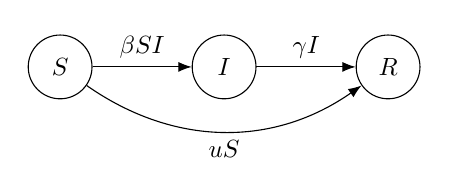
\begin{tikzpicture}[node distance=1.4cm,>=Latex,scale=0.9,transform shape]
\tikzstyle{state}=[circle,draw=black,minimum size=0.9cm,align=center]
\node[state] (S) {$S$};
\node[state,right=of S] (I) {$I$};
\node[state,right=of I] (R) {$R$};
\draw[->] (S) -- node[above] {$\beta S I$} (I);
\draw[->] (I) -- node[above] {$\gamma I$} (R);
\draw[->,bend right=35] (S) to node[below] {$uS$} (R);
\end{tikzpicture}
\end{center}

The diagram is often the easiest way to debug a model before coding. Every arrow should correspond to one or more terms in the ODE, and every ODE term should correspond to a meaningful arrow.

\subsection{SIR-style malware propagation}
A simple malware propagation model is
\begin{align}
    \dot{S} &= -\beta S I - u S,\label{eq:sir_s}\\
    \dot{I} &= \beta S I - \gamma I,\label{eq:sir_i}\\
    \dot{R} &= \gamma I + u S.\label{eq:sir_r}
\end{align}
Here:
\begin{itemize}[leftmargin=2em]
    \item $S(t)$ is the vulnerable/susceptible proportion;
    \item $I(t)$ is the infected/compromised proportion;
    \item $R(t)$ is the recovered/protected proportion;
    \item $\beta$ is the compromise rate;
    \item $\gamma$ is the recovery rate;
    \item $u(t)$ is a defense control, such as patching or hardening intensity.
\end{itemize}
The term $\beta S I$ means that vulnerable nodes become infected through contact with compromised nodes. The term $uS$ means that defense converts vulnerable nodes into protected nodes. This is a useful first example because it has few variables, interpretable parameters, and a conservation law
\begin{equation}
    S(t)+I(t)+R(t)=1.
\end{equation}

\subsection{APT compromise and repair model}
APT dynamics often involve compromise, persistence, detection, and repair. A minimal state vector is
\begin{equation}
    x(t)=[V(t),C(t),D(t),P(t)]^\top,
\end{equation}
where $V$ is vulnerable, $C$ is compromised but hidden, $D$ is detected, and $P$ is protected/repaired. A simple model is
\begin{align}
    \dot{V} &= -\beta V C - u_p V + \omega P,\\
    \dot{C} &= \beta V C - \alpha C - u_m C,\\
    \dot{D} &= \alpha C + u_m C - u_r D,\\
    \dot{P} &= u_p V + u_r D - \omega P.
\end{align}
Here $u_p$ is patching, $u_m$ is monitoring/detection, and $u_r$ is repair/remediation. This model is more relevant to APT defense because detection and repair are separated. A PINN can learn unknown rates such as $\beta$, $\alpha$, or $\omega$, and can also learn control functions $u_p(t),u_m(t),u_r(t)$.

\subsection{Rumor or misinformation propagation}
A simple misinformation model can use states
\begin{equation}
    x(t)=[U(t),M(t),C(t),F(t)]^\top,
\end{equation}
where $U$ is unaware, $M$ is misinformation spreader, $C$ is counter-message spreader, and $F$ is forgetting or inactive. One possible model is
\begin{align}
    \dot{U} &= -\beta_m U M -\beta_c U C + \delta F,\\
    \dot{M} &= \beta_m U M - \gamma M C - \eta_m M,\\
    \dot{C} &= \beta_c U C + \gamma M C - \eta_c C,\\
    \dot{F} &= \eta_m M + \eta_c C - \delta F.
\end{align}
This model distinguishes misinformation spreading from counter-messaging. If an intervention $u_c(t)$ represents fact-checking or education, then one may let
\begin{equation}
    \beta_c=\beta_{c0}+a_c u_c(t), \qquad \gamma=\gamma_0+a_\gamma u_c(t).
\end{equation}
This converts the model into a controlled system.

\begin{examplebox}{Choosing a PINN-ready model}
For a first PINN experiment, use the SIR malware model. For a second experiment, use the APT model because it has more compartments and multiple controls. For a social cyber-defense study, use the misinformation model. In all cases, write down the state variables, transition terms, unknown parameters, observed data, and conservation laws before designing the network.
\end{examplebox}

\section{Forward PINN: Solving a Known Propagation Model}

A forward PINN solves the model when parameters and controls are known. Although this is not the most exciting use of PINNs, it is the best way to debug the method.

For the malware model \eqref{eq:sir_s}-\eqref{eq:sir_r}, let
\begin{equation}
    [\hat{S}(t),\hat{I}(t),\hat{R}(t)]=N_x(t;\phi).
\end{equation}
The residuals are
\begin{align}
    r_S(t) &= \dot{\hat{S}} + \beta \hat{S}\hat{I} + u\hat{S},\\
    r_I(t) &= \dot{\hat{I}} - \beta \hat{S}\hat{I} + \gamma \hat{I},\\
    r_R(t) &= \dot{\hat{R}} - \gamma \hat{I} - u\hat{S}.
\end{align}
The loss is
\begin{equation}
    \mathcal{L}_{forward}=w_f\frac{1}{N_f}\sum_{j=1}^{N_f}(r_S^2+r_I^2+r_R^2)(t_j)+w_0\norm{\hat{x}(0)-x_0}^2+w_c\mathcal{L}_{cons},
\end{equation}
where
\begin{equation}
    \mathcal{L}_{cons}=\frac{1}{N_f}\sum_{j=1}^{N_f}\left(\hat{S}(t_j)+\hat{I}(t_j)+\hat{R}(t_j)-1\right)^2.
\end{equation}

A stronger parameterization enforces conservation automatically:
\begin{equation}
    [\hat{S},\hat{I},\hat{R}]=\softmax(N_x(t;\phi)).
\end{equation}
Then each component is positive and the three components sum to one. This can improve stability, but it also restricts the output form. Appendix \ref{app:constraints} discusses softmax and softplus transformations.

\section{Inverse PINN: Learning Unknown Propagation Parameters}

\subsection{Problem statement}
Suppose we observe only infected proportions
\begin{equation}
    \mathcal{D}=\{(t_i,I_i^{obs})\}_{i=1}^{N_d},
\end{equation}
and want to estimate $\beta$ and $\gamma$ in the malware model. A pure data-fitting approach may overfit or produce nonphysical trajectories. An inverse PINN uses both data and ODE residuals.

Let
\begin{equation}
    [\hat{S}(t),\hat{I}(t),\hat{R}(t)]=N_x(t;\phi), \qquad \hat{\beta},\hat{\gamma}\;\text{trainable}.
\end{equation}
The inverse PINN loss is
\begin{equation}
    \mathcal{L}_{inverse}=w_d\mathcal{L}_{data}+w_f\mathcal{L}_{ode}+w_0\mathcal{L}_{ic}+w_c\mathcal{L}_{cons}+w_p\mathcal{L}_{prior}.
\end{equation}
The data loss can be
\begin{equation}
    \mathcal{L}_{data}=\frac{1}{N_d}\sum_{i=1}^{N_d}\left(\hat{I}(t_i)-I_i^{obs}\right)^2.
\end{equation}
The ODE residuals use $\hat{\beta}$ and $\hat{\gamma}$:
\begin{align}
    r_S &= \dot{\hat{S}} + \hat{\beta}\hat{S}\hat{I}+u\hat{S},\\
    r_I &= \dot{\hat{I}} - \hat{\beta}\hat{S}\hat{I}+\hat{\gamma}\hat{I},\\
    r_R &= \dot{\hat{R}} - \hat{\gamma}\hat{I}-u\hat{S}.
\end{align}
If prior ranges are known, for example $\beta\in[0,2]$ and $\gamma\in[0,1]$, use constrained parameterization:
\begin{equation}
    \hat{\beta}=2\sigmoid(b_\beta),\qquad \hat{\gamma}=\sigmoid(b_\gamma),
\end{equation}
where $b_\beta,b_\gamma$ are unconstrained trainable scalars.

\subsection{Identifiability}
A parameter is identifiable if different parameter values produce distinguishably different observations. If only $I(t)$ is observed, then $\beta$ and $\gamma$ may be difficult to identify uniquely, especially over a short time window. This is not a PINN failure; it is a limitation of the inverse problem.

\begin{warningbox}
A small training loss does not automatically mean that the learned parameters are correct. Always report sensitivity checks: fit the model from multiple initial guesses, add noise, use different observation windows, and verify whether learned parameters are stable.
\end{warningbox}

\subsection{Observed states, hidden states, and auxiliary assumptions}
In cyber propagation, observations are rarely complete. We may observe only aggregate infected counts, while vulnerable, repaired, or counter-message states remain hidden. A PINN can infer hidden states only through the model structure and constraints. Therefore, the observation model should be stated explicitly:
\begin{equation}
    y^{obs}(t_i)=h(x(t_i))+\varepsilon_i,
\end{equation}
where $h$ maps the full state to the observed quantity. For example, $h(S,I,R)=I$ if only infection is observed, while $h(S,I,R)=N I$ if the data are infected counts in a population of size $N$.

\begin{longtable}{p{0.24\linewidth}p{0.34\linewidth}p{0.32\linewidth}}
\toprule
Observation case & PINN implication & Recommended validation \\
\midrule
All states observed & Parameter learning is easier & Compare every state trajectory \\
Only one compartment observed & Hidden states rely heavily on ODE constraints & Test multiple initial guesses and priors \\
Aggregated/noisy data & Need observation map $h(x)$ and noise-aware loss & Report robustness to noise and aggregation \\
No reliable data & PINN is mainly a solver under assumptions & Report sensitivity, not confident parameter recovery \\
\bottomrule
\end{longtable}

\subsection{A recommended workflow}
\begin{enumerate}[leftmargin=2em]
    \item Generate synthetic data from known parameters.
    \item Train the inverse PINN and verify that it recovers the known parameters.
    \item Reduce the number of observation points to test sparse-data behavior.
    \item Add noise to test robustness.
    \item Move to real or high-fidelity simulation data only after the synthetic test works.
\end{enumerate}

\section{PINN for Optimal Cyber Control}

Parameter learning answers ``what is the system?'' Optimal control answers ``what should the defender do?'' Consider
\begin{equation}
    \dot{x}=f(x,u,\theta,t),\qquad x(0)=x_0,
\end{equation}
with cost functional
\begin{equation}
    J(u)=\int_0^T L(x(t),u(t),t)\,\dd t+\Phi(x(T)).
\end{equation}
For malware defense, a typical cost is
\begin{equation}
    J(u)=\int_0^T \left[w_I I(t)+c_u u^2(t)\right]\dd t+w_T I(T).
\end{equation}
The defender wants low infection, but strong control is costly.

PINN-based control can be formulated in two main ways.

\subsection{Direct neural control PINN}
In direct control, use two networks:
\begin{equation}
    \hat{x}(t)=N_x(t;\phi), \qquad \hat{u}(t)=u_{\max}\sigmoid(N_u(t;\psi)).
\end{equation}
The sigmoid ensures $\hat{u}(t)\in[0,u_{\max}]$. The loss is
\begin{equation}
    \mathcal{L}_{direct}=w_J\widehat{J}+w_f\mathcal{L}_{ode}+w_0\mathcal{L}_{ic}+w_c\mathcal{L}_{constraint},
\end{equation}
where
\begin{equation}
    \widehat{J}=\frac{T}{N_f}\sum_{j=1}^{N_f}\left[w_I\hat{I}(t_j)+c_u\hat{u}^2(t_j)\right]+w_T\hat{I}(T).
\end{equation}
The ODE residual enforces system dynamics under $\hat{u}(t)$.

\begin{takeaway}
Direct neural control is simple and implementation-friendly. It learns an open-loop control function $u(t)$ directly. However, it may not satisfy the first-order optimality conditions unless the loss and optimization are strong enough.
\end{takeaway}

\subsection{PMP-informed PINN}
A PMP-informed PINN embeds the optimality system. This is more theoretically structured. For a minimization problem, define the Hamiltonian
\begin{equation}
    H(x,u,\lambda,t)=L(x,u,t)+\lambda^\top f(x,u,\theta,t),
\end{equation}
where $\lambda(t)$ is the costate variable. PMP gives
\begin{align}
    \dot{x} &= \frac{\partial H}{\partial \lambda}=f(x,u,\theta,t),\\
    \dot{\lambda} &= -\frac{\partial H}{\partial x},\\
    0 &= \frac{\partial H}{\partial u},\\
    x(0)&=x_0, \qquad \lambda(T)=\nabla_x\Phi(x(T)).
\end{align}
A PMP-informed PINN uses networks
\begin{equation}
    \hat{x}(t)=N_x(t;\phi),\qquad \hat{\lambda}(t)=N_\lambda(t;\eta),\qquad \hat{u}(t)=N_u(t;\psi),
\end{equation}
with loss
\begin{equation}
    \mathcal{L}_{PMP}=w_x\mathcal{L}_{state}+w_\lambda\mathcal{L}_{costate}+w_u\mathcal{L}_{stationarity}+w_b\mathcal{L}_{boundary}.
\end{equation}
The components are
\begin{align}
    \mathcal{L}_{state} &= \frac{1}{N_f}\sum_j\norm{\dot{\hat{x}}(t_j)-f(\hat{x}(t_j),\hat{u}(t_j),\theta,t_j)}^2,\\
    \mathcal{L}_{costate} &= \frac{1}{N_f}\sum_j\norm{\dot{\hat{\lambda}}(t_j)+\nabla_xH(\hat{x},\hat{u},\hat{\lambda},t_j)}^2,\\
    \mathcal{L}_{stationarity} &= \frac{1}{N_f}\sum_j\norm{\nabla_uH(\hat{x},\hat{u},\hat{\lambda},t_j)}^2,\\
    \mathcal{L}_{boundary} &= \norm{\hat{x}(0)-x_0}^2+\norm{\hat{\lambda}(T)-\nabla_x\Phi(\hat{x}(T))}^2.
\end{align}

\subsection{Example: PMP for SIR malware control}
For
\begin{align}
    \dot{S}&=-\beta SI-uS,\\
    \dot{I}&=\beta SI-\gamma I,\\
    \dot{R}&=\gamma I+uS,
\end{align}
with
\begin{equation}
    L=w_I I+c_u u^2,
\end{equation}
let $\lambda=[\lambda_S,\lambda_I,\lambda_R]^\top$. The Hamiltonian is
\begin{align}
H &= w_I I+c_u u^2 + \lambda_S(-\beta SI-uS) \\
&\quad + \lambda_I(\beta SI-\gamma I)+\lambda_R(\gamma I+uS).
\end{align}
The stationarity condition is
\begin{equation}
    \frac{\partial H}{\partial u}=2c_u u -\lambda_S S+\lambda_R S=0.
\end{equation}
Thus the unconstrained control is
\begin{equation}
    u^{raw}(t)=\frac{S(t)(\lambda_S(t)-\lambda_R(t))}{2c_u}.
\end{equation}
If $u(t)\in[0,u_{\max}]$, the projected control is
\begin{equation}
    u^*(t)=\min\{u_{\max},\max\{0,u^{raw}(t)\}\}.
\end{equation}
A PMP-informed PINN can either learn $u(t)$ directly and penalize the projected stationarity residual, or compute $u(t)$ from the learned state-costate variables using the above formula.

\begin{takeaway}
PMP-informed PINNs provide a strong connection between classical optimal control theory and neural computation. The network is not merely minimizing the cost; it is also asked to satisfy the state equation, costate equation, stationarity condition, and boundary conditions.
\end{takeaway}

\subsection{Direct control versus PMP-informed control}
The two approaches answer the same control question in different ways. Direct control treats the control as another neural output and optimizes the cost directly. PMP-informed control first derives the necessary optimality system and then asks the networks to satisfy that system.

\begin{longtable}{p{0.22\linewidth}p{0.34\linewidth}p{0.34\linewidth}}
\toprule
Aspect & Direct neural control PINN & PMP-informed PINN \\
\midrule
Main unknowns & $x(t)$ and $u(t)$ & $x(t)$, $u(t)$, and $\lambda(t)$ \\
Main objective & Minimize cost while satisfying dynamics & Satisfy PMP optimality system \\
Strength & Simple and flexible & Stronger theoretical structure \\
Weakness & May produce feasible but suboptimal control & More equations and harder training \\
Best first use & Debugging a control idea & Connecting with optimal control theory \\
Validation & Cost and baseline comparison & Residuals plus baseline comparison \\
\bottomrule
\end{longtable}

For a first paper or student project, it is usually wise to implement direct control first and then add the PMP-informed version as a more rigorous extension. If the two approaches produce similar control profiles, that agreement strengthens the result. If they disagree, the discrepancy should be investigated rather than hidden.

\section{PINN/PIDL under Sparse or Almost No Data}

\subsection{What PINNs can do with sparse data}
When only a small number of observations are available, a PINN can still use the differential equation residual as a learning signal. This is helpful when the model is trusted and observations are incomplete.

For example, suppose we observe infected nodes at only five time points. A purely data-driven neural network can interpolate these points in many unrealistic ways. A PINN constrains the interpolation to trajectories that approximately satisfy the malware ODE.

\subsection{What PINNs cannot do}
PINNs cannot create information that is absent from both data and model assumptions. If two parameter sets produce almost identical observed trajectories, then no method can reliably distinguish them without more information.

Therefore, in low-data cyber propagation studies, state clearly:
\begin{itemize}[leftmargin=2em]
    \item which parameters are learned from data;
    \item which parameters are fixed from domain knowledge;
    \item which parameters are regularized by prior ranges;
    \item which states are directly observed;
    \item which states are inferred only through the dynamics.
\end{itemize}

\subsection{Almost no data: a defensible use case}
If almost no data are available, use PINNs primarily as a \emph{physics-constrained solver}, not as evidence of true parameter recovery. A defensible workflow is:
\begin{enumerate}[leftmargin=2em]
    \item choose a mechanistic model based on domain reasoning;
    \item specify plausible parameter ranges;
    \item solve or control the model under those ranges;
    \item report sensitivity analysis rather than a single confident estimate;
    \item validate qualitatively or with future data when available.
\end{enumerate}

\begin{warningbox}
Avoid claiming that a PINN has ``discovered'' cyber propagation parameters from almost no data. A more accurate claim is that the PINN computes trajectories or controls consistent with the assumed model and parameter priors.
\end{warningbox}

\section{Game-Aware PINNs: Minimal Self-Contained Treatment}

Although this note is focused on PINNs, some cyber problems involve attackers and defenders. A two-player continuous-time game can be written as
\begin{equation}
    \dot{x}=f(x,u_A,u_D,\theta,t),
\end{equation}
where $u_A$ is the attack control and $u_D$ is the defense control. The attacker and defender may have different objectives:
\begin{align}
    J_A &= \int_0^T L_A(x,u_A,u_D,t)\dd t+\Phi_A(x(T)),\\
    J_D &= \int_0^T L_D(x,u_A,u_D,t)\dd t+\Phi_D(x(T)).
\end{align}

For an open-loop Nash equilibrium, each player has its own Hamiltonian:
\begin{align}
    H_A &= L_A+\lambda_A^\top f,\\
    H_D &= L_D+\lambda_D^\top f.
\end{align}
The PMP-style necessary conditions are
\begin{align}
    \dot{x} &= f(x,u_A,u_D),\\
    \dot{\lambda}_A &= -\nabla_x H_A,\\
    \dot{\lambda}_D &= -\nabla_x H_D,\\
    0 &= \nabla_{u_A}H_A,\\
    0 &= \nabla_{u_D}H_D.
\end{align}
A game-aware PINN can include all these residuals in the loss. However, this only gives a candidate equilibrium. It should be validated by unilateral deviation tests: can the attacker or defender improve their objective by changing only their own strategy?

\begin{takeaway}
For games, a small PINN residual is not enough. Report both residual quality and game-theoretic validation, such as approximate Nash gap or comparison against alternative strategies.
\end{takeaway}

\subsection{How game-aware PINNs differ from single-player PINNs}
The most important difference is that there is no single Hamiltonian in a general nonzero-sum game. Each player has a separate objective and therefore a separate Hamiltonian and costate. The shared state equation couples the players, but the stationarity condition is player-specific:
\begin{equation}
    \nabla_{u_A}H_A=0, \qquad \nabla_{u_D}H_D=0.
\end{equation}
In implementation, this means that a game-aware PINN loss should not simply minimize $J_A+J_D$ unless the game is intentionally reformulated as a cooperative problem. For attacker-defender games, minimizing a combined scalar loss may destroy the competitive meaning of Nash equilibrium. A clearer approach is to use the scalar training loss only as a numerical device that penalizes all players' residuals, while still reporting game-specific validation such as unilateral deviations.

\section{Hybrid and Impulsive Dynamics in a PINN Framework}

Cyber interventions are not always smooth. A patch campaign may continuously reduce vulnerability, while an emergency shutdown or awareness campaign may cause a sudden jump in state.

\subsection{Continuous control}
Continuous control means $u(t)$ affects the derivative over time:
\begin{equation}
    \dot{x}(t)=f(x(t),u(t),t).
\end{equation}
Here $u(t)$ is a function over an interval. In a PINN, represent $u(t)$ by a network or a parameterized function and include it in the residual.

\subsection{Sampled-data control without jump}
A defender may choose an action at decision times $t_k$, but the state does not jump:
\begin{equation}
    \dot{x}(t)=f(x(t),a_k,t), \qquad t\in[t_k,t_{k+1}),
\end{equation}
with
\begin{equation}
    x(t_k^+)=x(t_k^-).
\end{equation}
This is discrete decision-making with continuous evolution. A PINN can model it by using piecewise inputs or separate residuals on each interval.

\subsection{Impulsive control with jump}
Impulsive control means the state changes suddenly at selected times:
\begin{align}
    \dot{x}(t)&=f(x(t),u(t),t), \qquad t\ne \tau_i,\\
    x(\tau_i^+)&=G_i(x(\tau_i^-),v_i).
\end{align}
The function $G_i$ is the jump map, and $v_i$ is the impulse strength. The PINN loss should include both ODE residuals between impulses and jump residuals at impulse times:
\begin{equation}
    \mathcal{L}_{jump}=\sum_i \norm{\hat{x}(\tau_i^+)-G_i(\hat{x}(\tau_i^-),v_i)}^2.
\end{equation}

\subsection{Hybrid control}
Hybrid control combines a discrete mode with a continuous intensity. For example,
\begin{equation}
    a_k=(m_k,v_k), \qquad m_k\in\{\text{patch},\text{monitor},\text{isolate},\text{deceive}\},\quad v_k\in[0,1].
\end{equation}
If the mode only changes the derivative, use a piecewise ODE. If the mode causes an immediate jump, add a jump residual.

\begin{examplebox}{Hybrid misinformation intervention}
A continuous fact-checking effort changes the derivative by increasing counter-message adoption. A sudden platform announcement may instantly move a fraction of misinformation spreaders into the counter-message state. The first effect belongs in $f$; the second effect belongs in $G$.
\end{examplebox}


\section{PINN, PIDL, and Neural ODE: Clear Boundaries}

The terms PINN, PIDL, and Neural ODE are sometimes used together, but they play different roles.
\begin{itemize}[leftmargin=2em]
    \item \textbf{PINN:} the differential equation is mostly known. The neural network approximates the solution and is trained by equation residuals.
    \item \textbf{PIDL:} a broader term. It may include PINNs, neural operators, constrained loss functions, conservation-law penalties, and hybrid model-data architectures.
    \item \textbf{Neural ODE:} the derivative function itself is parameterized by a neural network, for example $\dot{x}=f_\theta(x,t)$. It is useful when the mechanism is unknown or partially unknown.
\end{itemize}

For cyber propagation, a practical distinction is the following:
\begin{equation}
\begin{array}{lll}
\text{Known mechanism, unknown solution} & \Rightarrow & \text{Forward PINN},\\
\text{Known mechanism, unknown parameters} & \Rightarrow & \text{Inverse PINN},\\
\text{Known mechanism, unknown control} & \Rightarrow & \text{Control PINN},\\
\text{Partially unknown mechanism} & \Rightarrow & \text{Hybrid PINN/Neural ODE},\\
\text{Data plus constraints plus priors} & \Rightarrow & \text{PIDL framework}.
\end{array}
\end{equation}

\begin{takeaway}
A pure PINN lecture should begin with the assumption that a differential equation model is available. Neural ODEs become central only when the model structure itself is uncertain. PIDL is the umbrella; PINN is one concrete and widely used implementation.
\end{takeaway}

\subsection{A fuller view of PIDL}
PIDL should be understood as a design space rather than a single algorithm. A PINN is one point in this design space: it approximates unknown functions by neural networks and penalizes differential-equation residuals. PIDL is broader. It asks how any available physical, cyber, or game-theoretic knowledge can be embedded into a deep learning pipeline.

In cyber propagation research, PIDL may include the following components.
\begin{enumerate}[leftmargin=2em]
    \item \textbf{Physics-informed residuals.} These are the standard PINN residuals such as
    \begin{equation}
        r(t)=\frac{\dd \hat{x}}{\dd t}-f(\hat{x},\hat{u},\hat{\theta},t).
    \end{equation}
    They state that the learned trajectory should obey the assumed cyber propagation law.
    \item \textbf{Conservation and feasibility constraints.} For example, compartment proportions should remain nonnegative and sum to one. This can be enforced by softmax parameterization or penalty terms.
    \item \textbf{Partially known mechanisms.} A cyber model may include a known part and an unknown correction:
    \begin{equation}
        \dot{x}=f_{\rm known}(x,u,\theta,t)+g_{\omega}(x,u,t).
    \end{equation}
    Here $g_{\omega}$ is a neural network that learns the missing mechanism. This is a PIDL model rather than a pure PINN, because the neural network is not only approximating the solution; it is also learning part of the dynamics.
    \item \textbf{Differentiable simulators.} Instead of enforcing only pointwise residuals, one can roll out a differentiable ODE solver and train through the simulation. This is useful when the model is more naturally written as a time-stepping simulator.
    \item \textbf{Optimality-informed constraints.} For control problems, PIDL can include PMP residuals, HJB/HJI residuals, budget constraints, or bounded-control KKT conditions.
    \item \textbf{Data-model fusion.} PIDL can combine sparse observations, synthetic simulator data, expert-generated FBSM trajectories, and prior ranges on parameters.
\end{enumerate}

\begin{longtable}{p{0.22\linewidth}p{0.33\linewidth}p{0.35\linewidth}}
\toprule
Setting & Better described as & Reason \\
\midrule
Known ODE, unknown state trajectory & Forward PINN & The equation is fixed and the network approximates the solution. \\
Known ODE, unknown parameters & Inverse PINN & Parameters are trainable variables constrained by the residual. \\
Known ODE, unknown control & Control PINN & The control is represented by a network and optimized with cost or PMP residuals. \\
Known ODE plus unknown correction term & PIDL / hybrid PINN-Neural ODE & The network learns missing physics/cyber mechanisms. \\
ODE solver embedded in training & PIDL / differentiable simulation & The constraint is enforced through rollout rather than only local residuals. \\
ODE plus PMP/HJB/game residuals & Game-aware or control-aware PIDL & The learning objective includes optimality or equilibrium conditions. \\
\bottomrule
\end{longtable}

\begin{takeaway}
Use the word PINN when the main object is a neural approximation trained by equation residuals. Use PIDL when the learning system also includes model correction terms, differentiable simulation, data assimilation, prior regularization, optimality residuals, or game-theoretic constraints. In a paper, it is better to state the exact residuals and constraints than to rely on the label alone.
\end{takeaway}


\section{From Cyber Model to PINN: A Seven-Step Translation}

A useful way to design a PINN project is to translate the original cyber problem into a learning problem step by step.

\begin{longtable}{p{0.12\linewidth}p{0.34\linewidth}p{0.42\linewidth}}
\toprule
Step & Question & Output \\
\midrule
1 & What are the compartments or states? & Define $x(t)$, e.g., $S,I,R$ or $V,C,D,P$. \\
2 & What mechanisms change the states? & Write each transition term in $f(x,u,\theta,t)$. \\
3 & What data are available? & Specify observed components, times, noise, and missing states. \\
4 & What is unknown? & Decide whether to learn states, parameters, controls, costates, or a missing mechanism. \\
5 & What constraints must hold? & Positivity, conservation, bounded controls, known parameter ranges. \\
6 & What residuals should be enforced? & ODE residuals, initial conditions, data loss, control optimality, jump residuals. \\
7 & How will success be validated? & Synthetic recovery, ODE solver comparison, sensitivity, baseline controls, Nash gap for games. \\
\bottomrule
\end{longtable}

\begin{center}
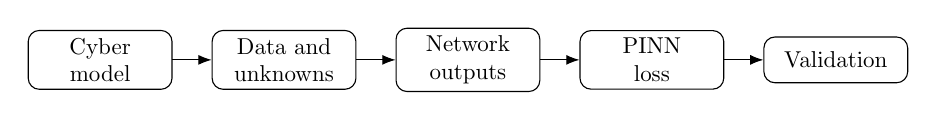
\begin{tikzpicture}[node distance=0.6cm,>=Latex,scale=0.83,transform shape]
\tikzstyle{box}=[rectangle,rounded corners,draw=black,align=center,minimum width=2.2cm,minimum height=0.7cm]
\node[box] (m) {Cyber\\model};
\node[box,right=of m] (d) {Data and\\unknowns};
\node[box,right=of d] (n) {Network\\outputs};
\node[box,right=of n] (l) {PINN\\loss};
\node[box,right=of l] (v) {Validation};
\draw[->] (m)--(d);\draw[->] (d)--(n);\draw[->] (n)--(l);\draw[->] (l)--(v);
\end{tikzpicture}
\end{center}

This translation is especially important when the PINN is used for optimal control. The network is not solving an abstract machine learning task; it is solving a constrained dynamical problem. Every loss term should correspond to a modeling statement.

\section{Worked Example 1: Sparse-Data Malware Parameter Learning}

Assume the true system is the malware SIR model
\begin{align}
    \dot{S}&=-\beta SI,\\
    \dot{I}&=\beta SI-\gamma I,\\
    \dot{R}&=\gamma I.
\end{align}
Only infected data $I^{obs}(t_i)$ are observed at a small number of time points. The goal is to learn $\beta$ and $\gamma$.

\subsection{Network design}
Use a state network
\begin{equation}
    z(t)=N_x(t;\phi)\in\R^3,
\end{equation}
and transform it into compartments by
\begin{equation}
    [\hat{S}(t),\hat{I}(t),\hat{R}(t)]=\softmax(z(t)).
\end{equation}
This automatically enforces positivity and conservation.

Use trainable scalars $b_\beta,b_\gamma$ and define
\begin{equation}
    \hat{\beta}=\beta_{\max}\sigmoid(b_\beta),\qquad
    \hat{\gamma}=\gamma_{\max}\sigmoid(b_\gamma).
\end{equation}
This prevents the optimizer from producing negative or unreasonably large rates.

\subsection{Loss construction}
The data loss is
\begin{equation}
    \mathcal{L}_{data}=\frac{1}{N_d}\sum_i(\hat{I}(t_i^d)-I_i^{obs})^2.
\end{equation}
The residual loss is
\begin{align}
    \mathcal{L}_{ode}=\frac{1}{N_f}\sum_j\big[& (\dot{\hat{S}}+\hat{\beta}\hat{S}\hat{I})^2
    +(\dot{\hat{I}}-\hat{\beta}\hat{S}\hat{I}+\hat{\gamma}\hat{I})^2 \\
    &+(\dot{\hat{R}}-\hat{\gamma}\hat{I})^2\big]_{t=t_j^f}.
\end{align}
If $x(0)$ is known, add
\begin{equation}
    \mathcal{L}_{ic}=\norm{\hat{x}(0)-x_0}^2.
\end{equation}
The total loss is
\begin{equation}
    \mathcal{L}=w_d\mathcal{L}_{data}+w_f\mathcal{L}_{ode}+w_0\mathcal{L}_{ic}.
\end{equation}

\subsection{What to report}
A clear report should show:
\begin{enumerate}[leftmargin=2em]
    \item the true and learned trajectories on synthetic data;
    \item the learned $\hat{\beta}$ and $\hat{\gamma}$ from several random initializations;
    \item performance when only 5, 10, or 20 observation points are used;
    \item performance under noisy observations;
    \item residual curves and data-fit curves separately.
\end{enumerate}

\section{Worked Example 2: PINN for APT Defense Control}

Consider the APT model
\begin{align}
    \dot{V} &= -\beta VC-u_pV+\omega P,\\
    \dot{C} &= \beta VC-\alpha C-u_mC,\\
    \dot{D} &= \alpha C+u_mC-u_rD,\\
    \dot{P} &= u_pV+u_rD-\omega P.
\end{align}
Suppose the defender wants to minimize
\begin{equation}
    J=\int_0^T\left[w_C C(t)+w_DD(t)+c_pu_p^2(t)+c_mu_m^2(t)+c_ru_r^2(t)\right]\dd t.
\end{equation}

\subsection{Direct control PINN formulation}
Use networks
\begin{equation}
    \hat{x}(t)=N_x(t;\phi),\qquad
    \hat{u}_p(t)=u_{p,\max}\sigmoid(N_p(t)),
\end{equation}
with analogous definitions for $\hat{u}_m$ and $\hat{u}_r$. The loss is
\begin{equation}
    \mathcal{L}=w_J\widehat{J}+w_f\mathcal{L}_{ode}+w_0\mathcal{L}_{ic}+w_c\mathcal{L}_{conservation}.
\end{equation}
This learns an open-loop defense schedule over time.

\subsection{PMP-informed formulation}
If one wants a stronger link with optimal control theory, add costate networks
\begin{equation}
    \hat{\lambda}(t)=N_\lambda(t;\eta)\in\R^4
\end{equation}
and include state, costate, stationarity, and boundary residuals. This is more difficult to train, but it gives a clearer connection to the classical optimality system.

\subsection{Practical interpretation}
The learned control curves should be interpreted as a cost-sensitive defense plan. A high $u_p$ early in the horizon means aggressive hardening; a high $u_m$ means intensive detection; a high $u_r$ means fast remediation. The cost terms prevent the PINN from selecting maximum defense all the time.

\section{Worked Example 3: Game-Aware PINN for Misinformation Defense}

A simplified attacker-defender misinformation game can be written as
\begin{equation}
    \dot{x}=f(x,u_A,u_D,\theta,t),
\end{equation}
where $u_A(t)$ is the misinformation amplification effort and $u_D(t)$ is the counter-message effort. Let the defender minimize
\begin{equation}
    J_D=\int_0^T\left[w_M M(t)+c_Du_D^2(t)\right]\dd t,
\end{equation}
and the attacker maximize
\begin{equation}
    J_A=\int_0^T\left[q_M M(t)-c_Au_A^2(t)\right]\dd t.
\end{equation}
A game-aware PINN can include:
\begin{itemize}[leftmargin=2em]
    \item one state network $N_x(t)$;
    \item one attacker control network $N_A(t)$;
    \item one defender control network $N_D(t)$;
    \item two costate networks $N_{\lambda_A}(t)$ and $N_{\lambda_D}(t)$;
    \item state residuals, two costate residuals, and two stationarity residuals.
\end{itemize}

The key validation is different from single-player control. Besides residual losses, report whether either player can improve by unilaterally changing its own strategy. This is an approximate Nash validation.



\section{How to Evaluate PINN/PIDL Performance}

Evaluation is often the weakest part of a PINN/PIDL study. A small training loss is not enough. A clear evaluation should answer: \emph{what is the reference}, \emph{what is being compared}, and \emph{what kind of claim is justified}. The reference may be true ground truth, a high-accuracy numerical solver, synthetic data, a benchmark control method, or consistency tests when no ground truth is available.

\subsection{Three evaluation regimes}
There are three common regimes.
\begin{enumerate}[leftmargin=2em]
    \item \textbf{Synthetic-data regime with ground truth.} We choose true parameters $\theta^\star$, solve the ODE with a reliable numerical solver, sample sparse/noisy observations, and ask whether the PINN/PIDL method can recover trajectories, parameters, or controls. This is the cleanest setting for method validation.
    \item \textbf{Real-data regime with partial observations.} True parameters and hidden states are unknown. Evaluation must rely on held-out observations, residual consistency, plausible parameter ranges, sensitivity analysis, and comparison against baseline models.
    \item \textbf{Almost-no-data regime.} There may be only initial conditions, prior parameter ranges, and the cyber mechanism. In this case, the model can generate a physics-consistent solution or control profile, but it cannot claim empirical parameter identification. The correct claim is feasibility, scenario exploration, or model-based control, not data-validated discovery.
\end{enumerate}

\subsection{What counts as ground truth?}
Ground truth can mean different things. It should be stated explicitly.
\begin{itemize}[leftmargin=2em]
    \item \textbf{Trajectory ground truth:} a known $x^\star(t)$ generated by an ODE solver or observed in a simulator/testbed.
    \item \textbf{Parameter ground truth:} known $\theta^\star$, usually available only in synthetic experiments.
    \item \textbf{Control ground truth:} an optimal or near-optimal control produced by FBSM, dynamic programming, exhaustive search in a small problem, or a trusted benchmark solver.
    \item \textbf{No ground truth:} use consistency, held-out prediction, robustness, and baseline comparison instead of claiming exact recovery.
\end{itemize}

\subsection{Metrics for forward and inverse PINNs}
For state prediction, report trajectory error on a dense validation grid:
\begin{equation}
    E_x=\left(\frac{1}{N}\sum_{j=1}^N \norm{\hat{x}(t_j)-x^{\star}(t_j)}_2^2\right)^{1/2}.
\end{equation}
For a single compartment such as compromised proportion $C(t)$, a useful metric is
\begin{equation}
    E_C=\left(\frac{1}{N}\sum_{j=1}^N |\hat{C}(t_j)-C^{\star}(t_j)|^2\right)^{1/2}.
\end{equation}
For parameter learning, use relative parameter error:
\begin{equation}
    E_\theta=\frac{\norm{\hat{\theta}-\theta^\star}_2}{\norm{\theta^\star}_2}.
\end{equation}
If $\theta^\star$ is not known, report confidence across random seeds, sensitivity to observation noise, and whether learned parameters lie in physically/cyber-plausible ranges.

\subsection{Metrics for control PINNs and PMP-informed PINNs}
For control, the main output is not only a trajectory but a decision policy or control function. Report the objective value
\begin{equation}
    J(\hat{u})=\int_0^T L(\hat{x}(t),\hat{u}(t),t)\dd t+\Phi(\hat{x}(T)),
\end{equation}
and compare it with baselines:
\begin{equation}
    J(\hat{u}) \quad \text{versus} \quad J(0),\; J(u_{\rm static}),\; J(u_{\rm threshold}),\; J(u_{\rm FBSM}).
\end{equation}
Also report the control effort $\int_0^T \hat{u}^2(t)\dd t$, peak infection or compromise level $\max_t C(t)$, and cumulative compromise $\int_0^T C(t)\dd t$.

For PMP-informed PINNs, include optimality residuals, not only ODE residuals:
\begin{equation}
    E_{\rm PMP}=\frac{1}{N}\sum_{j=1}^N\left(\norm{r_x(t_j)}_2^2+\norm{r_\lambda(t_j)}_2^2+\norm{r_u(t_j)}_2^2\right).
\end{equation}
A small state residual means the learned trajectory satisfies the dynamics. It does not necessarily mean the control is optimal. A small stationarity residual provides stronger evidence that the learned control satisfies PMP necessary conditions.

\subsection{Metrics for PIDL with unknown mechanisms}
If PIDL learns a missing mechanism $g_\omega$, evaluation should be more cautious. A learned correction term may fit data but still be non-identifiable. Recommended checks are:
\begin{enumerate}[leftmargin=2em]
    \item \textbf{Ablation:} compare the known-only model $f_{\rm known}$ with $f_{\rm known}+g_\omega$.
    \item \textbf{Held-out prediction:} fit on early times and test on later times, or fit on one initial condition and test on another.
    \item \textbf{Magnitude check:} verify whether $g_\omega$ is small and interpretable, or whether it dominates the known mechanism.
    \item \textbf{Robustness:} train with multiple seeds and noise levels; check whether the learned correction is stable.
\end{enumerate}

\subsection{A recommended evaluation ladder}
A strong tutorial or paper can use the following ladder.
\begin{longtable}{p{0.18\linewidth}p{0.34\linewidth}p{0.38\linewidth}}
\toprule
Level & Question & Evidence \\
\midrule
1 & Does the PINN solve the known ODE? & Compare with a high-accuracy ODE solver. \\
2 & Can it recover parameters from synthetic sparse data? & Parameter error and trajectory error against ground truth. \\
3 & Is it robust to noise and missing compartments? & Multiple noise levels, partial observations, random seeds. \\
4 & Does learned control improve the objective? & Compare $J$, peak infection, cumulative infection, and cost against baselines. \\
5 & Does it satisfy optimality or game conditions? & PMP residual, HJB/HJI residual, Nash-gap or unilateral-deviation tests. \\
6 & Does it generalize? & New initial conditions, new network sizes, unseen attack intensities. \\
\bottomrule
\end{longtable}

\begin{warningbox}
When no ground truth exists, avoid writing that the PINN ``accurately recovers'' the true parameters. Instead write that the learned parameters are consistent with observations, satisfy the governing equations, improve predictive performance on held-out data, or produce cost-effective controls under the assumed model.
\end{warningbox}

\section{Training Strategy and Diagnostics}

A clear PINN implementation is usually built in stages rather than all at once. The following staged strategy is useful for cyber propagation models.

\begin{enumerate}[leftmargin=2em]
    \item \textbf{Stage 1: forward sanity check.} Fix all parameters and controls. Train only the state network. Compare with an ODE solver. If this fails, do not proceed to parameter learning.
    \item \textbf{Stage 2: inverse parameter learning.} Make a small number of parameters trainable. Start with synthetic data where the true parameters are known. Verify recovery.
    \item \textbf{Stage 3: sparse/noisy data stress test.} Reduce observations and add noise. Report how parameter uncertainty increases.
    \item \textbf{Stage 4: control.} Add a control network or PMP-informed costate network. Compare against no control, static control, and a classical numerical method when available.
    \item \textbf{Stage 5: hybrid/game extension.} Add impulse residuals or player-wise optimality residuals only after the single-player continuous case is stable.
\end{enumerate}

\subsection{Diagnostics to plot}
A PINN paper should not show only the final trajectory. At minimum, plot:
\begin{itemize}[leftmargin=2em]
    \item total loss and each component loss separately;
    \item ODE residual over time after training;
    \item learned parameters across random seeds;
    \item state trajectories against data and ODE-solver baselines;
    \item for control, the learned control curve and the resulting cost components;
    \item for impulse systems, pre-jump and post-jump states around each impulse time.
\end{itemize}
These plots often reveal problems that a single loss number hides. For example, a low average residual may still have large residual spikes near sharp transitions.

\section{Implementation Roadmap}

\subsection{Step-by-step workflow}
A clean PINN project should follow the sequence below.
\begin{enumerate}[leftmargin=2em]
    \item \textbf{Model:} Define the state variables, ODEs, unknown parameters, controls, and constraints.
    \item \textbf{Data:} Specify which states are observed, at which times, and with what noise level.
    \item \textbf{Network outputs:} Decide whether the network outputs states only, states plus controls, or states plus controls plus costates.
    \item \textbf{Residuals:} Write explicit residual equations before coding.
    \item \textbf{Constraints:} Decide whether to enforce conservation/positivity by parameterization or penalties.
    \item \textbf{Training:} Start with Adam, optionally refine with L-BFGS. Monitor each loss component separately.
    \item \textbf{Validation:} Compare with an ODE solver, FBSM, synthetic ground truth, alternative parameter initializations, and sensitivity analysis.
\end{enumerate}

\subsection{Network architecture choices}
For one-dimensional time input, a typical state network is small:
\begin{equation}
    t \rightarrow \text{MLP}(4\text{--}6\text{ hidden layers}, 32\text{--}128\text{ neurons}) \rightarrow x(t).
\end{equation}
Use $\tanh$ activations initially. For stiff dynamics or sharp impulses, consider domain decomposition, adaptive collocation, or piecewise networks.


\subsection{Concrete neural-network setup}
This subsection gives a more operational description of how to set up the neural networks. The main design choice is not the number of layers. The main design choice is \emph{what mathematical object each network represents}. In a PINN/PIDL project, the neural networks should correspond directly to the unknown functions in the mathematical formulation.

\begin{longtable}{p{0.22\linewidth}p{0.24\linewidth}p{0.40\linewidth}}
\toprule
Network & Typical input/output & When to use it \\
\midrule
State network $N_x$ & $t \mapsto \hat{x}(t)$ & Forward and inverse PINNs. It approximates the trajectory of the propagation system. \\
Open-loop control network $N_u$ & $t \mapsto \hat{u}(t)$ & Continuous-time optimal control when the output is a planned control schedule over time. \\
Feedback control network $\pi_u$ & $(t,x) \mapsto \hat{u}(t,x)$ & Receding-horizon or policy-style control when the action should adapt to the observed state. \\
Costate network $N_\lambda$ & $t \mapsto \hat{\lambda}(t)$ & PMP-informed PINNs. It approximates the adjoint variables in the optimality system. \\
Correction network $N_c$ & $(t,x) \mapsto \hat{c}(t,x)$ & PIDL with missing mechanisms, for example unknown social amplification or unobserved attack pressure. \\
Parameter layer & trainable scalars $\hat{\theta}$ & Inverse PINNs. Raw parameters are transformed by softplus or sigmoid to satisfy physical ranges. \\
\bottomrule
\end{longtable}

\subsubsection*{Step 1: scale the input time}
Instead of feeding raw time $t\in[0,T]$ directly to the network, use
\begin{equation}
    \tau=\frac{t}{T}\in[0,1]
    \quad \text{or} \quad
    \tau=2\frac{t}{T}-1\in[-1,1].
\end{equation}
If the network is written as $\hat{x}(\tau)$, then the derivative must be converted correctly:
\begin{equation}
    \frac{\dd \hat{x}}{\dd t}=\frac{1}{T}\frac{\dd \hat{x}}{\dd \tau}.
\end{equation}
This small detail is a common source of implementation errors. If the time rescaling is ignored, the residual will enforce the wrong differential equation.

\subsubsection*{Step 2: choose the state output parameterization}
For compartment models, such as $S,I,R$ or $V,C,P$, states should usually be nonnegative and may need to sum to one. There are three common choices.
\begin{enumerate}[leftmargin=2em]
    \item \textbf{Unconstrained output plus penalty:}
    \begin{equation}
        \hat{x}(t)=N_x(t),\qquad
        \mathcal{L}_{constraint}=\sum_j \left(\sum_m \hat{x}_m(t_j)-1\right)^2+\sum_{m,j}\max(0,-\hat{x}_m(t_j))^2.
    \end{equation}
    This is flexible, but the network may produce negative states during training.
    \item \textbf{Softmax output:}
    \begin{equation}
        [\hat{S},\hat{I},\hat{R}]=\softmax(N_x(t)).
    \end{equation}
    This enforces positivity and conservation automatically, but it may make very small compartments hard to learn because softmax saturates.
    \item \textbf{Hard initial-condition output:}
    \begin{equation}
        \hat{x}(t)=x_0+t\,N_x(t).
    \end{equation}
    This enforces $\hat{x}(0)=x_0$ exactly. If time is scaled, use $\tau$ instead of $t$. This is useful when the initial state is known with high confidence.
\end{enumerate}

\subsubsection*{Step 3: choose control output parameterization}
For bounded control $u(t)\in[0,u_{\max}]$, use
\begin{equation}
    \hat{u}(t)=u_{\max}\sigmoid(N_u(t)).
\end{equation}
For multiple controls, apply this component-wise. If controls must satisfy a budget such as $u_1+u_2+u_3\leq B$, use either a penalty or a budget-preserving parameterization:
\begin{equation}
    [\hat{u}_1,\hat{u}_2,\hat{u}_3]=B\,\softmax(N_u(t)).
\end{equation}
The budget-preserving version is simple, but it forces the full budget to be spent. If unused budget is allowed, add an extra ``no-spend'' component to the softmax.

\subsubsection*{Step 4: choose trainable physical parameters}
Unknown parameters should not be left as arbitrary real numbers. For example,
\begin{equation}
    \hat{\beta}=\softplus(b_\beta)+10^{-6},\qquad
    \hat{\gamma}=\softplus(b_\gamma)+10^{-6}.
\end{equation}
If a parameter is a probability or efficacy in $[0,1]$, use
\begin{equation}
    \hat{\chi}=\sigmoid(b_\chi).
\end{equation}
If prior knowledge suggests $\beta\in[0.1,1.5]$, use
\begin{equation}
    \hat{\beta}=0.1+(1.5-0.1)\sigmoid(b_\beta).
\end{equation}
This makes the learned parameters physically meaningful and improves optimization.

\subsubsection*{Step 5: recommended default architectures}
The following defaults are good starting points, not universal rules.
\begin{longtable}{p{0.20\linewidth}p{0.28\linewidth}p{0.42\linewidth}}
\toprule
Component & Default architecture & Notes \\
\midrule
State network $N_x$ & 4 hidden layers, 64 neurons, $\tanh$ & Increase to 128 neurons for high-dimensional degree-based models. \\
Control network $N_u$ & 3 hidden layers, 32--64 neurons, $\tanh$ & Smooth control schedules usually need smaller networks than state trajectories. \\
Costate network $N_\lambda$ & Same size as state network & Costates may change sharply near terminal time; consider more collocation points near $T$. \\
Correction network $N_c$ & 2--3 hidden layers, 32 neurons & Keep small and regularized so that it does not replace the known physics. \\
Activation & $\tanh$ first & ReLU is less suitable when high-order derivatives are required. \\
Optimizer & Adam then L-BFGS & Adam explores; L-BFGS often improves residual accuracy. \\
\bottomrule
\end{longtable}

\subsubsection*{Step 6: decide whether the control is open-loop or feedback}
A time-only control network $N_u(t)$ learns an \emph{open-loop} schedule. It answers: ``What planned defense intensity should be used at each time?'' This is close to classical PMP/FBSM output.

A feedback control network $\pi_u(t,x)$ learns a policy that reacts to the current state. It answers: ``Given the current infection level or misinformation level, what defense action should be used?'' This is closer to RL and MPC. Feedback control usually needs data or simulation over many initial conditions, not just one trajectory.

\begin{takeaway}
For a first PINN control study, use $N_u(t)$ because it is simpler and comparable with PMP/FBSM. For a more deployable cyber-defense policy, use $\pi_u(t,x)$ and train across multiple initial conditions and parameter scenarios.
\end{takeaway}

\subsection{Implementation blueprint by task}
The following recipes translate the mathematical formulations into trainable modules.

\subsubsection*{Inverse PINN recipe}
\begin{enumerate}[leftmargin=2em]
    \item Define state network $N_x(t)$.
    \item Define trainable raw parameters $b_\beta,b_\gamma,\ldots$ and transform them into valid parameters.
    \item Sample data points $t_i^d$ and collocation points $t_j^f$.
    \item Compute $\hat{x}(t_i^d)$ for data loss.
    \item Compute $\frac{\dd \hat{x}}{\dd t}(t_j^f)$ by automatic differentiation.
    \item Compute ODE residual $r_j=\frac{\dd \hat{x}}{\dd t}(t_j^f)-f(\hat{x}(t_j^f),\hat{\theta},t_j^f)$.
    \item Minimize $\mathcal{L}_{data}+w_f\mathcal{L}_{ode}+w_0\mathcal{L}_{ic}+w_p\mathcal{L}_{prior}$.
\end{enumerate}

\subsubsection*{PIDL missing-mechanism recipe}
\begin{enumerate}[leftmargin=2em]
    \item Split the dynamics into known and unknown parts:
    \begin{equation}
        \dot{x}=f_{known}(x,u,\theta,t)+\epsilon N_c(t,x,u).
    \end{equation}
    \item Keep $N_c$ small and regularized:
    \begin{equation}
        \mathcal{L}_{corr}=\frac{1}{N_f}\sum_j \norm{N_c(t_j,x_j,u_j)}^2.
    \end{equation}
    \item Evaluate whether the correction improves held-out prediction or control performance. Do not interpret the correction as a real mechanism unless it is stable across data splits and parameter settings.
\end{enumerate}

\subsubsection*{Direct control PINN recipe}
\begin{enumerate}[leftmargin=2em]
    \item Define $N_x(t)$ and $N_u(t)$.
    \item Enforce control bounds by sigmoid or scaled sigmoid.
    \item Construct ODE residual using $\hat{u}(t)$.
    \item Approximate the objective by collocation quadrature:
    \begin{equation}
        J(\hat{u})\approx \frac{T}{N_f}\sum_{j=1}^{N_f} L(\hat{x}(t_j),\hat{u}(t_j),t_j)+\Phi(\hat{x}(T)).
    \end{equation}
    \item Minimize $J+w_f\mathcal{L}_{ode}+w_0\mathcal{L}_{ic}+w_c\mathcal{L}_{constraint}$.
\end{enumerate}

\subsubsection*{PMP-informed PINN recipe}
\begin{enumerate}[leftmargin=2em]
    \item Derive the Hamiltonian $H=L+\lambda^\top f$ on paper first.
    \item Define three networks: $N_x(t)$, $N_u(t)$, and $N_\lambda(t)$.
    \item Enforce the state residual $\dot{x}-\nabla_\lambda H$.
    \item Enforce the costate residual $\dot{\lambda}+\nabla_x H$.
    \item Enforce stationarity or projected stationarity for bounded controls.
    \item Enforce $x(0)=x_0$ and $\lambda(T)=\nabla_x\Phi(x(T))$.
\end{enumerate}
This formulation is more closely connected to classical optimal control than direct control PINN. It is also harder to train because state, costate, and control residuals can have very different scales.


\subsection{Loss scaling}
Always log individual loss terms:
\begin{equation}
    \mathcal{L}_{total}=w_d\mathcal{L}_{data}+w_f\mathcal{L}_{ode}+w_b\mathcal{L}_{boundary}+w_c\mathcal{L}_{constraint}+\cdots.
\end{equation}
If one term is many orders of magnitude larger than others, it may dominate training. Simple remedies include normalization, manual weights, curriculum training, or adaptive weighting \cite{wang2021lossimbalance}.

\section{Common Pitfalls and How to Avoid Them}

\begin{longtable}{p{0.26\linewidth}p{0.36\linewidth}p{0.30\linewidth}}
\toprule
Problem & Why it happens & Practical remedy \\
\midrule
ODE residual small but data fit poor & Physics loss dominates data loss & Increase $w_d$, normalize residuals, check observation noise \\
Data fit good but dynamics wrong & Data loss dominates residual loss & Increase $w_f$, add more collocation points \\
Negative compartments & Unconstrained network output & Use softmax/sigmoid output or positivity penalty \\
Parameters unrealistic & Unconstrained trainable parameters & Use softplus/sigmoid ranges and priors \\
Training unstable & Loss imbalance or stiff dynamics & Rescale time, normalize variables, use curriculum training \\
Control unrealistically aggressive & Cost weight too low & Increase control cost and enforce bounds \\
Claims too strong under sparse data & Identifiability not checked & Report sensitivity and multiple initializations \\
\bottomrule
\end{longtable}

\section{Reporting Checklist for a PINN Cyber Paper}
A complete PINN study should report the following.
\begin{enumerate}[leftmargin=2em]
    \item The exact ODE model and all state variables.
    \item Observed variables and observation times.
    \item Unknown parameters and their constraints/ranges.
    \item Network architecture and activation functions.
    \item Collocation sampling strategy.
    \item Full loss function with weights.
    \item Training optimizer, learning rate, and stopping criterion.
    \item Validation against synthetic data or numerical solvers.
    \item Sensitivity to noise, sparse data, and initialization.
    \item For control: comparison with no control, static control, FBSM, or other baselines.
    \item For games: unilateral deviation tests or approximate Nash gap.
\end{enumerate}

\newpage

\section{Python Implementation Map}
The companion code folder contains executable examples for the main PINN/PIDL tasks in this note.  The examples are designed to be readable and extendable.
\begin{longtable}{p{0.34\textwidth}p{0.56\textwidth}}
\toprule
Python file & PINN/PIDL task \\
\midrule
\texttt{inverse\_pinn\_sir\_malware.py} & inverse PINN: learn hidden states and unknown SIR parameters from sparse infection observations. \\
\texttt{pidl\_unknown\_mechanism.py} & PIDL correction: combine known SIR dynamics with a learned missing transfer term. \\
\texttt{control\_pinn\_malware.py} & direct neural-control PINN: train state and control networks by objective plus residual loss. \\
\texttt{pmp\_informed\_pinn\_malware.py} & PMP-informed PINN: train state, costate, and control networks with state, costate, stationarity, and boundary residuals. \\
\bottomrule
\end{longtable}
The separate running guide explains the exact commands, smoke tests, and troubleshooting steps.

\appendix


\section{Appendix A: Detailed Neural Network Setup Checklist}
\label{app:nnsetup}
This appendix summarizes the practical setup decisions that should be made before coding. It is intentionally concrete.

\subsection*{A.1 Inputs}
For trajectory learning, the input is usually normalized time $\tau\in[0,1]$ or $[-1,1]$. For feedback control, the input is $(\tau,x)$ or $(\tau,\hat{x})$. For PIDL corrections, the input is often $(\tau,x,u)$ because the missing mechanism may depend on both the state and the current intervention.

\subsection*{A.2 Outputs}
Choose outputs according to the unknown functions:
\begin{itemize}[leftmargin=2em]
    \item inverse PINN: output $\hat{x}(t)$; train $\hat{\theta}$;
    \item control PINN: output $\hat{x}(t)$ and $\hat{u}(t)$;
    \item PMP-informed PINN: output $\hat{x}(t)$, $\hat{u}(t)$, and $\hat{\lambda}(t)$;
    \item PIDL correction: output $\hat{x}(t)$ and a correction term $\hat{c}(t,x,u)$.
\end{itemize}

\subsection*{A.3 Architecture}
A practical default for ODE-based cyber propagation is:
\begin{equation}
    \text{MLP}(1,64,64,64,64,d_{out}) \quad \text{with } \tanh \text{ activations}.
\end{equation}
For high-dimensional degree-based models, increase width before increasing depth. For stiff or impulsive dynamics, a single global network may struggle; use piecewise networks, more collocation points near sharp changes, or a hybrid PINN with separate intervals.

\subsection*{A.4 Initialization}
Default Xavier initialization is usually sufficient. For inverse parameters, initialize raw parameters so that transformed values are near plausible priors. For example, if $\beta$ is expected near $0.5$, initialize $b_\beta$ such that $\softplus(b_\beta)\approx 0.5$. Bad parameter initialization can lead to a visually plausible trajectory but incorrect parameter recovery.

\subsection*{A.5 Training schedule}
A robust schedule is:
\begin{enumerate}[leftmargin=2em]
    \item Train with only data and initial condition losses for a short warm-up.
    \item Add the ODE residual loss.
    \item Add parameter priors or correction regularizers.
    \item For control, add the objective term only after the state residual is reasonably small.
    \item Optionally finish with L-BFGS.
\end{enumerate}
This curriculum is often more stable than optimizing the full loss from the first iteration.

\subsection*{A.6 What to print during training}
At regular intervals print:
\begin{equation}
    \mathcal{L}_{data},\quad \mathcal{L}_{ode},\quad \mathcal{L}_{ic},\quad \mathcal{L}_{constraint},\quad \hat{\theta},\quad \max_t |r_f(t)|.
\end{equation}
For control problems also print $J$, peak infection, cumulative infection, and total control effort. If the total loss decreases but one critical component increases, the final result may be misleading.

\section{Appendix B: Neural Network Basics}
A multilayer perceptron (MLP) is a composition of affine transformations and nonlinear activations. For PINNs, the input is often time $t$ or space-time $(x,t)$, and the output is a state approximation. Smooth activations such as $\tanh$ are usually preferred because PINNs require derivatives of network outputs.

\section{Appendix C: Automatic Differentiation}
\label{app:autodiff}
Automatic differentiation computes derivatives of network outputs with respect to inputs. If $I_\phi(t)$ is a neural network output, then a deep learning library can compute
\begin{equation}
    \frac{\dd I_\phi(t)}{\dd t}
\end{equation}
without finite differences. This is crucial because the ODE residual uses derivatives at collocation points.

\section{Appendix D: Collocation Point Sampling}
Collocation points can be sampled uniformly, randomly, or adaptively. Uniform sampling is simple and often sufficient for smooth dynamics. Adaptive sampling places more points where the residual is large or where the trajectory changes rapidly. For impulsive systems, sample separately in each interval between impulse times and include points near the jumps.

\section{Appendix E: Constrained Outputs and Parameters}
\label{app:constraints}
\subsection{Softmax for compartment conservation}
For compartments that must be nonnegative and sum to one, use
\begin{equation}
    [\hat{S},\hat{I},\hat{R}]=\softmax([z_S,z_I,z_R]),
\end{equation}
where
\begin{equation}
    \softmax(z_i)=\frac{e^{z_i}}{\sum_k e^{z_k}}.
\end{equation}
This enforces $\hat{S}+\hat{I}+\hat{R}=1$ and each component is positive.

\subsection{Sigmoid for bounded controls}
To enforce $u(t)\in[0,u_{\max}]$, use
\begin{equation}
    \hat{u}(t)=u_{\max}\sigmoid(z(t)),\qquad \sigmoid(z)=\frac{1}{1+e^{-z}}.
\end{equation}

\subsection{Softplus for positive parameters}
To enforce $\beta>0$, use
\begin{equation}
    \hat{\beta}=\softplus(b)=\log(1+e^b).
\end{equation}
If a known upper bound exists, use a scaled sigmoid instead.


\section{Appendix F: Optimizers for PINN Training}
PINN training often uses two stages. First, Adam is used because it is robust and easy to tune. Second, L-BFGS is used to refine the solution because it often reduces residual errors more effectively near a local minimum. A common schedule is:
\begin{equation}
    \text{Adam for }10^4\text{--}10^5\text{ iterations} \quad \rightarrow \quad \text{L-BFGS refinement}.
\end{equation}
There is no universal best schedule. The important point is to monitor each loss component separately. If the ODE residual decreases while the data loss increases, the loss weights may be poorly balanced.

\section{Appendix G: Normalization and Non-dimensionalization}
PINNs are sensitive to scale. If time ranges from 0 to 10,000 while states range from 0 to 1, gradients may become poorly conditioned. A simple transformation is
\begin{equation}
    \tau=\frac{t}{T}\in[0,1].
\end{equation}
Then
\begin{equation}
    \frac{\dd x}{\dd t}=\frac{1}{T}\frac{\dd x}{\dd \tau}.
\end{equation}
The ODE residual must be written consistently after rescaling. State variables, parameters, and costs should also be normalized when their magnitudes differ significantly.

\section{Appendix H: ODE Solvers and PINNs}
An ODE solver propagates a state forward step by step. Euler's method is
\begin{equation}
    x_{k+1}=x_k+\Delta t f(x_k,u_k,t_k).
\end{equation}
The fourth-order Runge-Kutta method is more accurate and uses four slope evaluations per step. PINNs do not need to use an ODE solver inside the residual, because derivatives are obtained by automatic differentiation. However, ODE solvers remain useful for generating synthetic data and validating learned trajectories.

\section{Appendix I: Minimal PMP Recap}
For a minimization problem
\begin{equation}
    \min_u \int_0^T L(x,u,t)\dd t+\Phi(x(T)),\qquad \dot{x}=f(x,u,t),
\end{equation}
PMP introduces the Hamiltonian
\begin{equation}
    H=L+\lambda^\top f.
\end{equation}
The necessary conditions are
\begin{align}
    \dot{x}&=\nabla_\lambda H,\\
    \dot{\lambda}&=-\nabla_x H,\\
    0&=\nabla_u H,\\
    x(0)&=x_0,\qquad \lambda(T)=\nabla_x\Phi(x(T)).
\end{align}
A PMP-informed PINN turns these equations into residuals and trains neural networks to satisfy them.

\section{Appendix J: Minimal Pseudo-Code}
\begin{lstlisting}
Choose model: dx/dt = f(x,u,theta,t)
Choose networks: x_hat(t), optionally u_hat(t), lambda_hat(t)
Choose trainable parameters: theta_hat
Sample data points and collocation points
For each training iteration:
    evaluate x_hat at data and collocation points
    use autodiff to compute dx_hat/dt
    compute ODE residuals
    compute data, IC/BC, constraint losses
    if control: compute cost loss or PMP residuals
    combine losses with weights
    update neural-network weights and trainable parameters
Validate:
    compare with ODE solver or known synthetic truth
    check residuals, parameter stability, and sensitivity
\end{lstlisting}

\section{Appendix K: Choosing Network Outputs}
The output layer should reflect the mathematical structure of the problem. For unconstrained states, a linear output is acceptable. For compartments that are proportions, a softmax output is often better. For controls bounded in $[0,u_{\max}]$, a sigmoid-scaled output is natural. For positive physical parameters, use softplus or a scaled sigmoid.

\begin{longtable}{p{0.24\linewidth}p{0.30\linewidth}p{0.34\linewidth}}
\toprule
Quantity & Recommended output & Reason \\
\midrule
State proportions summing to one & Softmax over raw logits & Enforces positivity and conservation \\
Single bounded state & Scaled sigmoid & Enforces lower and upper bounds \\
Positive rate parameter & Softplus or scaled sigmoid & Avoids negative transition rates \\
Open-loop control & Small MLP with sigmoid output & Produces a smooth bounded function of time \\
Costate variable & Linear output & Costates can be positive or negative \\
Piecewise/impulse state & Separate networks per interval or time-feature encoding & Avoids forcing a smooth network across jumps \\
\bottomrule
\end{longtable}

\section{Appendix L: A Minimal PINN Experiment Template}
A reproducible experiment can be described by the following template.
\begin{enumerate}[leftmargin=2em]
    \item \textbf{Model.} Write the ODEs and list every parameter with units or interpretation.
    \item \textbf{Data.} State which compartments are observed and how noise is generated or measured.
    \item \textbf{Unknowns.} Declare whether the unknowns are states, parameters, controls, costates, or impulse strengths.
    \item \textbf{Network.} Give input variables, output variables, activation, width, depth, and output transformations.
    \item \textbf{Residuals.} Write each residual explicitly. Do not rely on verbal descriptions only.
    \item \textbf{Training.} Report optimizer, learning rate, iterations, collocation points, and loss weights.
    \item \textbf{Validation.} Compare with ground truth, numerical solvers, baselines, sensitivity tests, or Nash-gap tests.
\end{enumerate}

\section{Appendix M: Glossary of Common Terms}
\begin{longtable}{p{0.24\linewidth}p{0.66\linewidth}}
\toprule
Term & Meaning in this note \\
\midrule
Forward problem & Solve the state trajectory when model and parameters are known. \\
Inverse problem & Learn unknown parameters or hidden states from observations. \\
Collocation point & A point where the equation residual is enforced, even without observed data. \\
Physics residual & Mismatch between neural derivative and the differential equation. \\
Hard constraint & A constraint enforced by parameterization, such as softmax conservation. \\
Soft constraint & A constraint enforced by a penalty term in the loss. \\
Open-loop control & A control represented as a function of time over the horizon. \\
Feedback control & A control represented as a function of the current state. \\
Impulse & A discrete event that causes an instantaneous jump in the state. \\
Hybrid control & A combination of continuous evolution, discrete modes, and possibly impulses. \\
Identifiability & Whether parameters can be uniquely inferred from the available observations and model. \\
\bottomrule
\end{longtable}


\section{Appendix N: Python Example 1 - Inverse PINN for SIR Malware Propagation}
This example illustrates a minimal inverse PINN. It generates synthetic sparse data from an SIR-style malware model, then learns the state trajectory and two unknown parameters. The example is intentionally compact. For a serious experiment, add train/validation splits, multiple seeds, noise experiments, and plots.

\begin{lstlisting}[language=Python]
# Inverse PINN for SIR-style malware propagation.
# Requirements: torch, numpy, matplotlib.
import math
import numpy as np
import torch
import torch.nn as nn

DEVICE = "cuda" if torch.cuda.is_available() else "cpu"
torch.manual_seed(1)

# ---------- 1. Synthetic ground truth ----------
def sir_rhs(x, beta, gamma):
    S, I, R = x[..., 0], x[..., 1], x[..., 2]
    dS = -beta * S * I
    dI = beta * S * I - gamma * I
    dR = gamma * I
    return torch.stack([dS, dI, dR], dim=-1)

def rk4_step(x, dt, beta, gamma):
    k1 = sir_rhs(x, beta, gamma)
    k2 = sir_rhs(x + 0.5 * dt * k1, beta, gamma)
    k3 = sir_rhs(x + 0.5 * dt * k2, beta, gamma)
    k4 = sir_rhs(x + dt * k3, beta, gamma)
    return x + dt * (k1 + 2*k2 + 2*k3 + k4) / 6.0

def generate_data(beta_true=0.8, gamma_true=0.2, T=20.0, n_grid=400):
    dt = T / (n_grid - 1)
    t = torch.linspace(0, T, n_grid).view(-1, 1)
    x = torch.zeros(n_grid, 3)
    x[0] = torch.tensor([0.95, 0.05, 0.0])
    for k in range(n_grid - 1):
        x[k+1] = rk4_step(x[k], dt, beta_true, gamma_true)
        x[k+1] = torch.clamp(x[k+1], 0.0, 1.0)
        x[k+1] = x[k+1] / x[k+1].sum()
    return t, x

t_all, x_all = generate_data()
# Sparse observations: only I(t) is observed at 30 times.
idx = torch.linspace(0, len(t_all)-1, 30).long()
t_data = t_all[idx].to(DEVICE)
I_data = x_all[idx, 1:2].to(DEVICE)

# ---------- 2. PINN model ----------
class StateNet(nn.Module):
    def __init__(self, width=64, depth=4):
        super().__init__()
        layers = [nn.Linear(1, width), nn.Tanh()]
        for _ in range(depth - 1):
            layers += [nn.Linear(width, width), nn.Tanh()]
        layers += [nn.Linear(width, 3)]
        self.net = nn.Sequential(*layers)
    def forward(self, t):
        logits = self.net(t)
        # Softmax enforces S,I,R >= 0 and S+I+R = 1.
        return torch.softmax(logits, dim=-1)

model = StateNet().to(DEVICE)
# Raw trainable parameters. Softplus enforces positivity.
beta_raw = nn.Parameter(torch.tensor(0.0, device=DEVICE))
gamma_raw = nn.Parameter(torch.tensor(-1.0, device=DEVICE))
params = list(model.parameters()) + [beta_raw, gamma_raw]
opt = torch.optim.Adam(params, lr=1e-3)

def positive(raw):
    return torch.nn.functional.softplus(raw) + 1e-6

# Collocation points where the ODE residual is enforced.
T = 20.0
t_f = torch.linspace(0, T, 200).view(-1, 1).to(DEVICE)
t_f.requires_grad_(True)
x0 = torch.tensor([[0.95, 0.05, 0.0]], device=DEVICE)

# ---------- 3. Training loop ----------
for it in range(8000):
    opt.zero_grad()
    beta = positive(beta_raw)
    gamma = positive(gamma_raw)

    # Data loss: only I(t) is observed.
    x_d = model(t_data)
    loss_data = torch.mean((x_d[:, 1:2] - I_data)**2)

    # Initial condition loss.
    x_init = model(torch.zeros(1, 1, device=DEVICE))
    loss_ic = torch.mean((x_init - x0)**2)

    # ODE residual loss through automatic differentiation.
    x_f = model(t_f)
    grads = []
    for j in range(3):
        grad_j = torch.autograd.grad(
            x_f[:, j].sum(), t_f, create_graph=True
        )[0]
        grads.append(grad_j)
    dxdt = torch.cat(grads, dim=1)
    rhs = sir_rhs(x_f, beta, gamma)
    loss_ode = torch.mean((dxdt - rhs)**2)

    loss = loss_data + 10.0 * loss_ic + loss_ode
    loss.backward()
    opt.step()

    if it % 1000 == 0:
        print(it, float(loss), float(beta), float(gamma))

print("learned beta, gamma =", float(positive(beta_raw)), float(positive(gamma_raw)))

# Evaluation with synthetic ground truth.
with torch.no_grad():
    t_eval = t_all.to(DEVICE)
    x_pred = model(t_eval).cpu()
    rmse_I = torch.sqrt(torch.mean((x_pred[:, 1] - x_all[:, 1])**2))
    print("I(t) RMSE against ground truth =", float(rmse_I))
\end{lstlisting}

\section{Appendix O: Python Example 2 - PIDL with a Missing Propagation Mechanism}
This example shows the PIDL idea. The known model is SIR, but we add a small neural correction to the infected equation. This is useful when the classical model is plausible but incomplete. Evaluation must check whether the correction improves held-out prediction and remains stable across seeds.

\begin{lstlisting}[language=Python]
# PIDL example: known SIR model plus a learned correction term.
# This is a template. It assumes x_hat(t) is produced by a state network.
import torch
import torch.nn as nn

class CorrectionNet(nn.Module):
    def __init__(self, width=32):
        super().__init__()
        self.net = nn.Sequential(
            nn.Linear(4, width), nn.Tanh(),
            nn.Linear(width, width), nn.Tanh(),
            nn.Linear(width, 1)
        )
    def forward(self, t, x):
        # Input includes time and current learned state [S,I,R].
        return self.net(torch.cat([t, x], dim=1))

def pidl_rhs(t, x, beta, gamma, corr_net, eps=0.1):
    S, I, R = x[:, 0:1], x[:, 1:2], x[:, 2:3]
    base_dS = -beta * S * I
    base_dI = beta * S * I - gamma * I
    base_dR = gamma * I
    correction = eps * torch.tanh(corr_net(t, x))
    # The correction adds to dI. To preserve S+I+R, subtract it from dS.
    dS = base_dS - correction
    dI = base_dI + correction
    dR = base_dR
    return torch.cat([dS, dI, dR], dim=1)

# In the training loss, replace the pure SIR residual by:
# residual = d_x_hat_dt - pidl_rhs(t_f, x_hat, beta, gamma, corr_net)
# loss_ode = mean(residual**2)
# Add a regularizer to avoid an arbitrary large correction:
# loss_corr = mean(corr_net(t_f, x_hat)**2)
# total_loss = data_loss + ic_loss + ode_loss + alpha_corr * loss_corr

# Why regularize the correction?
# Without regularization, the neural correction may explain everything and
# the known cyber mechanism becomes irrelevant. A small correction is easier
# to interpret and more likely to generalize.
\end{lstlisting}

\section{Appendix P: Python Example 3 - Direct Neural Control PINN}
This example outlines a direct control PINN. The state network learns $S,I,R$ and the control network learns $u(t)$. The training objective combines ODE residuals and the control cost. This direct approach is easier to code than a PMP-informed PINN, but it does not explicitly enforce costate equations or stationarity conditions.

\begin{lstlisting}[language=Python]
# Direct neural control PINN for controlled malware SIR dynamics.
import torch
import torch.nn as nn

class ControlNet(nn.Module):
    def __init__(self, umax=1.0, width=32):
        super().__init__()
        self.umax = umax
        self.net = nn.Sequential(
            nn.Linear(1, width), nn.Tanh(),
            nn.Linear(width, width), nn.Tanh(),
            nn.Linear(width, 1)
        )
    def forward(self, t):
        # Bounded patching intensity u(t) in [0, umax].
        return self.umax * torch.sigmoid(self.net(t))

def controlled_sir_rhs(x, u, beta, gamma):
    S, I, R = x[:, 0:1], x[:, 1:2], x[:, 2:3]
    dS = -beta*S*I - u*S
    dI = beta*S*I - gamma*I
    dR = gamma*I + u*S
    return torch.cat([dS, dI, dR], dim=1)

# Suppose state_net(t) gives softmax-normalized [S,I,R].
# Suppose control_net(t) gives u(t).
# At collocation points t_f:
#   x = state_net(t_f)
#   u = control_net(t_f)
#   dxdt = autodiff_derivative(x, t_f)
#   residual = dxdt - controlled_sir_rhs(x, u, beta, gamma)
#   loss_ode = mean(residual**2)
#   running_cost = wI * x[:,1:2] + cu * u**2
#   loss_cost = mean(running_cost) + wT * x_T[:,1:2]
#   total_loss = loss_ode + alpha_ic * loss_ic + alpha_cost * loss_cost
# Then optimize state_net and control_net jointly.

# Evaluation:
# 1. Roll out the learned u(t) with an independent ODE solver.
# 2. Compare J(u) with no control, static control, threshold control,
#    and FBSM if available.
# 3. Report peak infection, cumulative infection, and total control effort.
\end{lstlisting}

\section{Appendix Q: Python Example 4 - PMP-Informed Residual Skeleton}
This skeleton shows how the PMP-informed idea differs from direct control. In addition to the state network and control network, one adds a costate network and penalizes costate and stationarity residuals.

\begin{lstlisting}[language=Python]
# PMP-informed PINN skeleton for controlled SIR.
# Variables: x=[S,I,R], control u, costate lambda=[lS,lI,lR].
# Hamiltonian H = wI*I + cu*u^2 + lambda^T f(x,u).

def hamiltonian(x, u, lam, beta, gamma, wI=10.0, cu=0.1):
    f = controlled_sir_rhs(x, u, beta, gamma)
    running = wI * x[:, 1:2] + cu * u**2
    return running + torch.sum(lam * f, dim=1, keepdim=True)

# At collocation points t_f:
# x = state_net(t_f), u = control_net(t_f), lam = costate_net(t_f)
# H = hamiltonian(x, u, lam, beta, gamma)
#
# State residual:
#   r_x = d_x_dt - dH_dlambda, equivalent to d_x_dt - f(x,u)
# Costate residual:
#   r_lam = d_lam_dt + dH_dx
# Stationarity residual:
#   r_u = dH_du
# Terminal residual:
#   lambda(T) - grad Phi(x(T))
#
# total_loss = loss_state + loss_costate + loss_stationarity
#              + loss_initial + loss_terminal
#
# For bounded controls, exact stationarity may become a KKT condition.
# A practical approximation is to use sigmoid-bounded u(t), or penalize
# the projected gradient instead of raw dH/du.
\end{lstlisting}



\section{Appendix R: Python Example 5 - Modular PINN/PIDL Building Blocks}
This example gives modular building blocks rather than a full experiment. It shows how to set up state networks, control networks, costate networks, correction networks, and constrained trainable parameters. These classes can be reused in the earlier examples.

\begin{lstlisting}[language=Python]
import torch
import torch.nn as nn
import torch.nn.functional as F

class MLP(nn.Module):
    """Small smooth MLP for PINN/PIDL components."""
    def __init__(self, in_dim, out_dim, width=64, depth=4, act=nn.Tanh):
        super().__init__()
        layers = [nn.Linear(in_dim, width), act()]
        for _ in range(depth - 1):
            layers += [nn.Linear(width, width), act()]
        layers += [nn.Linear(width, out_dim)]
        self.net = nn.Sequential(*layers)
        self.reset_parameters()

    def reset_parameters(self):
        for m in self.net:
            if isinstance(m, nn.Linear):
                nn.init.xavier_normal_(m.weight)
                nn.init.zeros_(m.bias)

    def forward(self, x):
        return self.net(x)

class CompartmentStateNet(nn.Module):
    """State network for SIR/VCP-type compartments.
    The softmax output enforces positivity and conservation.
    """
    def __init__(self, n_states=3, width=64, depth=4):
        super().__init__()
        self.backbone = MLP(1, n_states, width, depth)

    def forward(self, tau):
        logits = self.backbone(tau)
        return F.softmax(logits, dim=-1)

class HardICStateNet(nn.Module):
    """State network with hard initial condition x(0)=x0.
    It uses x(tau)=x0+tau*N(tau). Add softmax only if needed.
    """
    def __init__(self, x0, n_states=3, width=64, depth=4):
        super().__init__()
        self.register_buffer("x0", torch.as_tensor(x0).float().view(1, -1))
        self.net = MLP(1, n_states, width, depth)

    def forward(self, tau):
        return self.x0 + tau * self.net(tau)

class BoundedControlNet(nn.Module):
    """Open-loop control u(tau) in [umin, umax]."""
    def __init__(self, n_controls=1, umin=0.0, umax=1.0, width=32, depth=3):
        super().__init__()
        self.umin, self.umax = umin, umax
        self.net = MLP(1, n_controls, width, depth)

    def forward(self, tau):
        raw = self.net(tau)
        return self.umin + (self.umax - self.umin) * torch.sigmoid(raw)

class FeedbackControlNet(nn.Module):
    """Feedback control pi(tau,x) in [umin,umax]."""
    def __init__(self, n_states, n_controls=1, umin=0.0, umax=1.0,
                 width=64, depth=3):
        super().__init__()
        self.umin, self.umax = umin, umax
        self.net = MLP(1 + n_states, n_controls, width, depth)

    def forward(self, tau, x):
        raw = self.net(torch.cat([tau, x], dim=1))
        return self.umin + (self.umax - self.umin) * torch.sigmoid(raw)

class CostateNet(nn.Module):
    """Costate lambda(tau). Usually unconstrained."""
    def __init__(self, n_states=3, width=64, depth=4):
        super().__init__()
        self.net = MLP(1, n_states, width, depth)

    def forward(self, tau):
        return self.net(tau)

class CorrectionNet(nn.Module):
    """PIDL correction c(tau,x,u), kept small and regularized."""
    def __init__(self, n_states, n_controls=0, out_dim=1, width=32, depth=2):
        super().__init__()
        self.net = MLP(1 + n_states + n_controls, out_dim, width, depth)

    def forward(self, tau, x, u=None):
        if u is None:
            u = torch.empty((tau.shape[0], 0), device=tau.device)
        return self.net(torch.cat([tau, x, u], dim=1))

class PositiveParameter(nn.Module):
    """Trainable positive scalar parameter via softplus."""
    def __init__(self, init_value=0.5):
        super().__init__()
        raw = torch.log(torch.exp(torch.tensor(float(init_value))) - 1.0)
        self.raw = nn.Parameter(raw.clone().detach())

    def forward(self):
        return F.softplus(self.raw) + 1e-6

class BoundedParameter(nn.Module):
    """Trainable scalar parameter in [low, high]."""
    def __init__(self, low=0.0, high=1.0, init_value=0.5):
        super().__init__()
        self.low, self.high = low, high
        z = (init_value - low) / (high - low)
        z = min(max(z, 1e-4), 1 - 1e-4)
        raw = torch.log(torch.tensor(z / (1 - z)))
        self.raw = nn.Parameter(raw.float())

    def forward(self):
        return self.low + (self.high - self.low) * torch.sigmoid(self.raw)

def d_dt(y, tau, T=1.0):
    """Derivative dy/dt when tau=t/T. y has shape [N,d]."""
    grads = []
    for k in range(y.shape[1]):
        g = torch.autograd.grad(y[:, k].sum(), tau, create_graph=True)[0]
        grads.append(g / T)
    return torch.cat(grads, dim=1)

# Typical assembly for a PMP-informed control PINN:
# state_net = CompartmentStateNet(n_states=3)
# control_net = BoundedControlNet(n_controls=1, umax=1.0)
# costate_net = CostateNet(n_states=3)
# beta = PositiveParameter(0.6)
# gamma = PositiveParameter(0.2)
# params = (list(state_net.parameters()) + list(control_net.parameters()) +
#           list(costate_net.parameters()) + list(beta.parameters()) +
#           list(gamma.parameters()))
# optimizer = torch.optim.Adam(params, lr=1e-3)
\end{lstlisting}

\section{Appendix S: Practical Hyperparameter Starting Points}
\begin{longtable}{p{0.28\linewidth}p{0.24\linewidth}p{0.40\linewidth}}
\toprule
Item & Starting value & Comment \\
\midrule
Time scaling & $t/T$ to $[0,1]$ & Always account for derivative scaling. \\
State network & 4 layers, 64 neurons & Increase width for high-dimensional states. \\
Activation & $\tanh$ & Smooth and usually stable for ODE residuals. \\
Collocation points & 200--1000 for ODEs & Increase near rapid transitions or impulses. \\
Learning rate & $10^{-3}$ for Adam & Reduce to $10^{-4}$ if losses oscillate. \\
Initial-condition weight & 10--100 & Use hard IC if the initial condition is exact. \\
ODE residual weight & 1 initially & Increase after warm-up if dynamics are violated. \\
Correction regularization & $10^{-3}$--$10^{-1}$ & Larger values force corrections to be smaller. \\
Control cost weight & problem dependent & Tune so that the learned control is not always maximal. \\
Random seeds & at least 5 & Essential for parameter-identifiability claims. \\
\bottomrule
\end{longtable}

\section{Appendix T: Implementation Debugging Checklist}
Before trusting a result, check the following.
\begin{enumerate}[leftmargin=2em]
    \item Does the forward PINN reproduce a known ODE-solver trajectory when parameters are fixed?
    \item If time is normalized, is the derivative scaled by $1/T$?
    \item Are all compartments nonnegative and, when required, do they sum to one?
    \item Are learned parameters constrained to physically meaningful ranges?
    \item Are individual loss components logged separately?
    \item Does the model work on synthetic data before being used on real data?
    \item Does the result remain similar under multiple random seeds?
    \item For PIDL corrections, does the correction remain small and interpretable?
    \item For control, is the learned control evaluated by an independent ODE solver rather than only by the training residual?
    \item For PMP-informed PINNs, are state, costate, stationarity, initial, and terminal residuals all checked separately?
\end{enumerate}


\newpage
\begin{thebibliography}{99}
\bibitem{raissi2019pinn} M. Raissi, P. Perdikaris, and G. E. Karniadakis, ``Physics-informed neural networks: A deep learning framework for solving forward and inverse problems involving nonlinear partial differential equations,'' \emph{Journal of Computational Physics}, vol. 378, pp. 686--707, 2019.
\bibitem{karniadakis2021pinnreview} G. E. Karniadakis, I. G. Kevrekidis, L. Lu, P. Perdikaris, S. Wang, and L. Yang, ``Physics-informed machine learning,'' \emph{Nature Reviews Physics}, vol. 3, pp. 422--440, 2021.
\bibitem{lu2021deepxde} L. Lu, X. Meng, Z. Mao, and G. E. Karniadakis, ``DeepXDE: A deep learning library for solving differential equations,'' \emph{SIAM Review}, vol. 63, no. 1, pp. 208--228, 2021.
\bibitem{sirignano2018dgm} J. Sirignano and K. Spiliopoulos, ``DGM: A deep learning algorithm for solving partial differential equations,'' \emph{Journal of Computational Physics}, vol. 375, pp. 1339--1364, 2018.
\bibitem{chen2018neuralode} R. T. Q. Chen, Y. Rubanova, J. Bettencourt, and D. Duvenaud, ``Neural ordinary differential equations,'' in \emph{Advances in Neural Information Processing Systems}, 2018.
\bibitem{wang2021lossimbalance} S. Wang, Y. Teng, and P. Perdikaris, ``Understanding and mitigating gradient flow pathologies in physics-informed neural networks,'' \emph{SIAM Journal on Scientific Computing}, vol. 43, no. 5, pp. A3055--A3081, 2021.
\bibitem{krishnapriyan2021pinnfailures} A. Krishnapriyan, A. Gholami, S. Zhe, R. Kirby, and M. W. Mahoney, ``Characterizing possible failure modes in physics-informed neural networks,'' in \emph{Advances in Neural Information Processing Systems}, 2021.
\bibitem{lenhart2007optimal} S. Lenhart and J. T. Workman, \emph{Optimal Control Applied to Biological Models}. Chapman and Hall/CRC, 2007.
\bibitem{kirk2004optimal} D. E. Kirk, \emph{Optimal Control Theory: An Introduction}. Dover, 2004.
\bibitem{cheng2024hodge} X. Cheng, L.-X. Yang, Q. Zhu, C. Gan, X. Yang, and G. Li, ``Cost-effective hybrid control strategies for dynamical propaganda war game,'' \emph{IEEE Transactions on Information Forensics and Security}, vol. 19, pp. 9789--9802, 2024.
\bibitem{jafar2024malware} M. T. Jafar, L.-X. Yang, G. Li, Q. Zhu, and C. Gan, ``Minimizing malware propagation in Internet of Things networks: An optimal control using feedback loop approach,'' \emph{IEEE Transactions on Information Forensics and Security}, vol. 19, pp. 9682--9697, 2024.
\bibitem{yang2019apt} L.-X. Yang, P. Li, X. Yang, Y. Y. Tang, and Y. Y. Tang, ``Security evaluation of the cyber networks under advanced persistent threats,'' \emph{IEEE Transactions on Dependable and Secure Computing}, vol. 16, no. 5, pp. 892--906, 2019.
\end{thebibliography}


\end{document}
